% ============================================================
% METHODOLOGY
% SAR: STATE AWARE RETRIEVAL FOR ITERATIVE
% RETRIEVAL-AUGMENTED GENERATION
%
% COMPILER:
% pdfLaTeX
%
% REQUIRED FILES:
% image1.png (college logo), gantt_chart.png (Gantt chart)
% ============================================================

\documentclass[12pt,a4paper]{report}

% ============================================================
% FONT
% ============================================================

\usepackage{newtxtext,newtxmath}

% ============================================================
% PAGE SIZE AND MARGINS
% ============================================================

\usepackage[
    a4paper,
    top=0.66in,
    bottom=0.66in,
    left=0.78in,
    right=0.78in
]{geometry}

% ============================================================
% PACKAGES
% ============================================================

\usepackage{setspace}
\usepackage{graphicx}
\usepackage{array}
\usepackage{booktabs}
\usepackage{longtable}
\usepackage{tabularx}
\usepackage{ragged2e}
\usepackage{amsmath}
\usepackage{tikz}\usetikzlibrary{positioning,fit,calc,shapes.geometric}
\usepackage{eso-pic}
\usepackage{fancyhdr}
\usepackage{tocloft}
\usepackage{hyperref}
\usepackage{enumitem}
\usepackage{float}
\usepackage[table]{xcolor}
\usepackage{etoolbox}

% TikZ styles used in the methodology architecture
\tikzset{
    block/.style={
        rectangle,
        draw,
        rounded corners,
        align=center,
        minimum width=28mm,
        minimum height=8mm
    },
    important/.style={
        rectangle,
        draw,
        rounded corners,
        align=center,
        minimum width=32mm,
        minimum height=9mm
    },
    arrow/.style={
        ->,
        >=stealth,
        thick
    }
}
\makeatletter
\patchcmd{\thebibliography}
  {\chapter*{\bibname}}
  {}
  {}
  {}
\makeatother

\newcommand{\figplaceholder}[4]{%
\begin{figure}[H]
\centering
\IfFileExists{#1}{\includegraphics[width=0.92\textwidth]{#1}}{%
\fbox{\parbox[c][#2][c]{0.88\textwidth}{\centering\small [ Insert figure: \detokenize{#1} ]}}}
\caption{#3}
\label{fig:#4}
\end{figure}}

% ============================================================
% GENERAL FORMATTING
% ============================================================

\setlength{\parindent}{0pt}
\setlength{\parskip}{0pt}
\AtBeginDocument{\setlength{\parindent}{0pt}}

\onehalfspacing

\hypersetup{
    colorlinks=false,
    hidelinks
}

% ============================================================
% PAGE BORDER
%
% Border is deliberately inside the physical page edge.
% It is applied to EVERY page.
% ============================================================

\AddToShipoutPictureBG{%
    \begin{tikzpicture}[remember picture,overlay]
        \draw[line width=0.5pt]
        ([xshift=0.30in,yshift=-0.30in]current page.north west)
        rectangle
        ([xshift=-0.30in,yshift=0.30in]current page.south east);
    \end{tikzpicture}%
}

% ============================================================
% HEADER / FOOTER
%
% Department name:
% TOP RIGHT
% SLIGHTLY ABOVE THE PAGE BORDER
%
% Page number:
% CENTERED
% SLIGHTLY RAISED FROM BOTTOM
% ============================================================

\pagestyle{fancy}

\fancyhf{}

% ------------------------------------------------------------
% Department name -- top right
% ------------------------------------------------------------

\fancyhead[R]{%
    \raisebox{0.22in}{%
        \fontsize{10}{12}\selectfont
        Department of Computer Engineering
    }%
}

% ------------------------------------------------------------
% Page number -- centered and raised
% ------------------------------------------------------------

\fancyfoot[C]{%
    \raisebox{0.18in}{%
        \fontsize{10}{12}\selectfont
        \thepage
    }%
}

% ------------------------------------------------------------
% Remove header/footer lines
% ------------------------------------------------------------

\renewcommand{\headrulewidth}{0pt}
\renewcommand{\footrulewidth}{0pt}

% ------------------------------------------------------------
% Header height
% ------------------------------------------------------------

\setlength{\headheight}{15pt}


% ============================================================
% CHAPTER-OPENING PAGES
%
% LaTeX normally changes chapter-opening pages to the
% "plain" style. Make it identical to the normal page style.
% ============================================================

\fancypagestyle{plain}{
    \fancyhf{}

    % Department name -- top right
    \fancyhead[R]{%
        \raisebox{0.22in}{%
            \fontsize{10}{12}\selectfont
            Department of Computer Engineering
        }%
    }

    % Page number -- centered and raised
    \fancyfoot[C]{%
        \raisebox{0.18in}{%
            \fontsize{10}{12}\selectfont
            \thepage
        }%
    }

    \renewcommand{\headrulewidth}{0pt}
    \renewcommand{\footrulewidth}{0pt}
}

% ============================================================
% HEADING FONT SIZES (Times New Roman style)
%   normal text   : 12 pt
%   subsubsection : 12 pt bold
%   subsection    : 14 pt bold  (sub-topic)
%   section       : 16 pt bold  (main topic)
%   chapter title : 22 pt bold, right aligned
% ============================================================

\makeatletter
\renewcommand\section{\@startsection{section}{1}{\z@}%
    {-3.5ex \@plus -1ex \@minus -.2ex}%
    {2.3ex \@plus.2ex}%
    {\normalfont\fontsize{16}{19}\selectfont\bfseries}}
\renewcommand\subsection{\@startsection{subsection}{2}{\z@}%
    {-3.25ex\@plus -1ex \@minus -.2ex}%
    {1.5ex \@plus .2ex}%
    {\normalfont\fontsize{14}{17}\selectfont\bfseries}}
\renewcommand\subsubsection{\@startsection{subsubsection}{3}{\z@}%
    {-3.25ex\@plus -1ex \@minus -.2ex}%
    {1.5ex \@plus .2ex}%
    {\normalfont\fontsize{12}{15}\selectfont\bfseries}}
\makeatother

% ============================================================
% TITLE COMMANDS
% ============================================================

\newcommand{\fronttitle}[1]{
    \begin{center}
        {\fontsize{18}{21}\selectfont\bfseries #1\par}
    \end{center}
    \vspace{0.12in}
}

\newcommand{\chaptertitle}[2]{
    \begin{flushright}
        {\fontsize{22}{26}\selectfont\bfseries CHAPTER #1\par}
        \vspace{0.10in}
        {\fontsize{22}{26}\selectfont\bfseries #2\par}
    \end{flushright}
    \vspace{0.12in}
}

% Right-aligned main title without a chapter number (used for REFERENCES)
\newcommand{\righttitle}[1]{
    \begin{flushright}
        {\fontsize{22}{26}\selectfont\bfseries #1\par}
    \end{flushright}
    \vspace{0.12in}
}

% ============================================================
% DOCUMENT
% ============================================================

\begin{document}

% PAGE 1 -- TITLE PAGE
% ============================================================

\begin{titlepage}
\thispagestyle{empty}
\begin{center}

\vspace*{0.58in}

{\fontsize{16}{19}\selectfont\bfseries
SAR: State Aware Retrieval\\for Iterative Retrieval Augmented Generation\par}

\vspace{0.18in}

{\fontsize{12}{18}\selectfont
A Project Report Submitted in\par}
\vspace{0.12in}
{\fontsize{12}{18}\selectfont
partial fulfillment of requirements for the degree of\par}
\vspace{0.12in}
{\fontsize{12}{18}\selectfont
Bachelor of Technology\par}
\vspace{0.10in}
{\fontsize{12}{18}\selectfont\bfseries\itshape
In\par}
\vspace{0.08in}
{\fontsize{12}{18}\selectfont
Computer Engineering\par}
\vspace{0.10in}
{\fontsize{12}{18}\selectfont\bfseries\itshape
By\par}
\vspace{0.08in}
{\fontsize{12}{18}\selectfont
Kunal Dahal (22CSEC17)\par
Aniket Manger (22CSEC23)\par
Suman Chettri (22CSEC44)\par}

\vspace{0.10in}

{\fontsize{12}{18}\selectfont\itshape
Under the supervision of\par}
\vspace{0.06in}
{\fontsize{14}{17}\selectfont\bfseries
Mr. Anmol Pandey\par}
\vspace{0.04in}
{\fontsize{12}{18}\selectfont
Assistant Professor\par}
\vspace{0.04in}
{\fontsize{12}{18}\selectfont
Computer Engineering Department\par}
\vspace{0.12in}

\IfFileExists{image1.png}{
\includegraphics[width=0.82in]{image1.png}}{\fbox{\rule{0pt}{0.82in}\rule{0.82in}{0pt}}}

\vspace{0.10in}
{\fontsize{14}{17}\selectfont\bfseries
Department Of Computer Engineering\par}
\vspace{0.04in}
{\fontsize{14}{17}\selectfont\bfseries
Sikkim Institute of Science and Technology\par}
\vspace{0.04in}
{\fontsize{14}{17}\selectfont\bfseries
(A constituent college of Sikkim University)\par}
\vspace{0.04in}
{\fontsize{14}{17}\selectfont\bfseries
2026\par}

\end{center}
\end{titlepage}

% ============================================================
\pagenumbering{roman}

% PAGE 2 -- ABSTRACT
% ============================================================

\fronttitle{ABSTRACT}
\justifying

Retrieval Augmented Generation (RAG) uses external documents to help large language models answer complex questions. However, during iterative retrieval, documents that are relevant to the original question may repeat information that has already been retrieved, while other required information is still missing. This leads to redundant retrieval and incomplete evidence collection.

This project proposes \textbf{State Aware Retrieval (SAR)} for iterative RAG. SAR uses a Sentence Transformer to represent the question, information gaps, collected evidence, and documents in a common semantic space. Based on these representations, a state aware scoring equation assigns a score to every document. The equation combines three factors: relevance to the original question, coverage of the current information gap, and novelty with respect to the evidence already collected. This allows retrieval to consider both what is relevant to the question and what information is still required. The documents are then ranked by their final scores, and the Top-$K$ documents with the highest scores are selected for the next retrieval step. SAR therefore selects documents according to the current retrieval state instead of relying only on the original question.

The proposed approach aims to reduce redundant retrieval and to select more complementary evidence for complex question answering. Its effectiveness will be studied through a systematic evaluation of retrieval quality and answer quality.

\vspace{0.10in}
\textbf{Keywords:} Retrieval Augmented Generation, Information Retrieval, Iterative Retrieval, Multi-Hop Question Answering.
\clearpage

% ============================================================

% PAGE 3
% TABLE OF CONTENTS
% ============================================================

\fronttitle{TABLE OF CONTENTS}

\begin{center}

\renewcommand{\arraystretch}{1.45}

\makebox[\textwidth][c]{%
\begin{tabular}{|>{\centering\arraybackslash}p{0.55in}|
                >{\centering\arraybackslash}p{5.5in}|
                >{\centering\arraybackslash}p{0.55in}|}
\hline
\textbf{CHP NO.} & \textbf{TOPICS} & \textbf{PAGE NO.} \\
\hline
& ABSTRACT & i \\
\hline
& TABLE OF CONTENTS & ii \\
\hline
& LIST OF TABLES & \pageref{lot} \\
\hline
& LIST OF FIGURES & \pageref{lof} \\
\hline
1. & INTRODUCTION & \pageref{ch:1} \\
\hline
2. & LITERATURE SURVEY & \pageref{ch:2}--\pageref{ch:2:end} \\
\hline
3. & PROBLEM DEFINITION & \pageref{ch:3} \\
\hline
4. & OBJECTIVES & \pageref{ch:4} \\
\hline
5. & METHODOLOGY & \pageref{ch:5}--\pageref{ch:5:end} \\
\hline
6. & SOFTWARE AND HARDWARE REQUIREMENTS & \pageref{ch:6}--\pageref{ch:6:end} \\
\hline
7. & IMPLEMENTATION & \pageref{ch:7}--\pageref{ch:7:end} \\
\hline
8. & APPLICATIONS & \pageref{ch:8} \\
\hline
9. & GANTT CHART & \pageref{ch:9} \\
\hline
10. & CONCLUSION & \pageref{ch:10} \\
\hline
& REFERENCES & \pageref{ch:refs} \\
\hline
\end{tabular}%
}

\end{center}
\clearpage



% ============================================================


% PAGE 4
% LIST OF TABLES AND FIGURES
% ============================================================

\fronttitle{LIST OF TABLES}
\label{lot}

\begin{center}

\renewcommand{\arraystretch}{1.35}

\makebox[\textwidth][c]{%
\begin{tabular}{|>{\centering\arraybackslash}p{0.85in}|
                >{\centering\arraybackslash}p{4.95in}|
                >{\centering\arraybackslash}p{0.75in}|}

\hline
\textbf{TABLE NO.} & \textbf{TITLE} & \textbf{PAGE NO.} \\
\hline
2.1 & Literature Survey 1 & \pageref{tab:lit1} \\
\hline
2.2 & Literature Survey 2 & \pageref{tab:lit2} \\
\hline
2.3 & Literature Survey 3 & \pageref{tab:lit3} \\
\hline
2.4 & Literature Survey 4 & \pageref{tab:lit4} \\
\hline
2.5 & Literature Survey 5 & \pageref{tab:lit5} \\
\hline
5.1 & State Aware Retrieval Configuration & \pageref{tab:sar-settings} \\
\hline
5.2 & State Aware Retrieval Hyperparameters & \pageref{tab:sar-hyperparameters} \\
\hline
5.3 & Models used in SAR, MIGRES, and baseline systems & \pageref{tab:models} \\
\hline
5.4 & Information Retrieval Baseline Comparison & \pageref{tab:baseline-comparison} \\
\hline
6.1 & Software Requirements & \pageref{tab:software-requirements} \\
\hline
6.2 & Modules Description & \pageref{tab:module-description} \\
\hline
7.1 & Hardware Environment & \pageref{tab:hardware-environment} \\
\hline
7.2 & Software Environment & \pageref{tab:software-environment} \\
\hline
7.3 & Experiment Notebooks and Their Mapping to the Experimental Design & \pageref{tab:impl-notebooks} \\
\hline
7.4 & Outputs Saved for Each Experimental Run & \pageref{tab:impl-output-files} \\
\hline
\end{tabular}%
}

\end{center}

\clearpage

\fronttitle{LIST OF FIGURES}
\label{lof}

\begin{center}

\renewcommand{\arraystretch}{1.35}

\makebox[\textwidth][c]{%
\begin{tabular}{|>{\centering\arraybackslash}p{0.95in}|
                >{\centering\arraybackslash}p{4.85in}|
                >{\centering\arraybackslash}p{0.75in}|}

\hline
\textbf{FIGURE NO.} & \textbf{TITLE} & \textbf{PAGE NO.} \\
\hline
5.1 & Architecture of State Aware Retrieval & \pageref{fig:sar-architecture} \\
\hline
5.2 & Operational Flow of State Aware Retrieval & \pageref{fig:sar-flow} \\
\hline
7.1 & Overall System Implementation Flow & \pageref{fig:system-implementation} \\
\hline
7.2 & Corpus Preparation and Embedding Pipeline & \pageref{fig:impl-corpus-flow} \\
\hline
7.3 & MIGRES State and Processing Flow with SAR Integration & \pageref{fig:migres-state-processing} \\
\hline
7.4 & Architecture of the SAR Retrieval Module & \pageref{fig:sar-module} \\
\hline
7.5 & Project Structure of the SAR--MIGRES Implementation & \pageref{fig:project-structure} \\
\hline
7.6 & Code-Level Architecture of the SAR--MIGRES Implementation & \pageref{fig:code-level-architecture} \\
\hline
7.7 & Implementation of the SAR Scoring and Retrieval Module & \pageref{fig:sar-scoring-retrieval-module} \\
\hline
9.1 & Gantt Chart & \pageref{fig:gantt} \\
\hline
\end{tabular}%
}

\end{center}
\clearpage



% ============================================================


% CHAPTER 1 -- INTRODUCTION
% ============================================================

\pagenumbering{arabic}
\setcounter{page}{1}
\addcontentsline{toc}{chapter}{1. INTRODUCTION}
\chaptertitle{1}{INTRODUCTION}
\label{ch:1}
\justifying

Retrieval Augmented Generation (RAG) is a technique that combines information retrieval with large language models to improve question answering. Instead of depending only on the information stored inside a language model, RAG retrieves relevant information from external documents and uses it to generate an answer \cite{lewis2020rag}. This makes RAG useful for tasks where the required information is spread across different documents.

However, answering complex questions is not as simple as finding documents that are related to the question. Some questions need several pieces of information, and the first retrieval step may provide only part of what is required. Multi-hop question answering benchmarks and iterative retrieval methods show that such questions can require evidence from multiple passages or documents and repeated retrieval steps \cite{yang2018hotpotqa,trivedi2022musique,yadav2020iterative}. If the retrieval system keeps selecting documents mainly because they are related to the original question, it may retrieve similar information again and again instead of finding the missing evidence.

\textbf{MIGRES (Missing Information Guided Retrieve-Extraction-Solving)} provides a framework for handling this type of iterative information retrieval. It keeps track of the information already collected and identifies the information that is still required to answer the question \cite{wang2025migres}. This creates an opportunity to improve the retrieval stage by considering not only the original question, but also the current information gap and the evidence already collected. Related work on relevant information gain also supports reducing redundant evidence while preserving useful information for RAG \cite{pickett2024better}.

This project proposes State Aware Retrieval (SAR), a retrieval method that improves document selection in such iterative RAG systems. The main idea is to select documents based on three things: their relevance to the question, their usefulness for covering the missing information, and the amount of new information they provide compared with the evidence already collected.

The proposed approach will be studied within the MIGRES framework and evaluated on question-answering datasets. The overall aim of this project is to examine whether making the retrieval process aware of the current information state can help RAG systems retrieve more useful and complementary evidence for complex questions.

\clearpage

% ============================================================
% CHAPTER 2 -- LITERATURE SURVEY
% ============================================================

\setcounter{table}{0}
\renewcommand{\thetable}{2.\arabic{table}}
\renewcommand{\theHtable}{chapter2.\arabic{table}}
\setcounter{figure}{0}
\renewcommand{\thefigure}{2.\arabic{figure}}
\renewcommand{\theHfigure}{chapter2.\arabic{figure}}

\addcontentsline{toc}{chapter}{2. LITERATURE SURVEY}
\chaptertitle{2}{LITERATURE SURVEY}
\label{ch:2}
\justifying

% ------------------------------------------------------------
% PAPER 1
% ------------------------------------------------------------
\begin{longtable}{|p{1.25in}|p{5.15in}|}
\caption{Literature Survey 1}\label{tab:lit1}\\
\hline
\hline
\textbf{Name of paper} & Retrieval-Augmented Generation for Knowledge-Intensive NLP Tasks \cite{lewis2020rag} \\ \hline

\textbf{Authors} & Patrick Lewis, Ethan Perez, Aleksandra Piktus, Fabio Petroni, Vladimir Karpukhin, Naman Goyal, Heinrich K\"uttler, Mike Lewis, Wen-tau Yih, Tim Rockt\"aschel, Sebastian Riedel, and Douwe Kiela \\ \hline

\textbf{Publication Details} & Advances in Neural Information Processing Systems 33 (NeurIPS), 2020, pp. 9459--9474. \\ \hline

\textbf{Research Findings} &
\begin{itemize}[leftmargin=0.18in,itemsep=0.05in,topsep=0pt,parsep=0pt]
\item RAG combines information stored in a language model with information retrieved from external documents.
\item Retrieved passages help the model answer questions that require outside knowledge.
\item The approach shows that retrieval can improve the performance of language generation for knowledge-intensive tasks.
\item The work provides a basic foundation for modern retrieval-augmented generation systems.
\end{itemize} \\ \hline

\textbf{Research Gap} &
\begin{itemize}[leftmargin=0.18in,itemsep=0.05in,topsep=0pt,parsep=0pt]
\item RAG searches for documents only once, using the input question alone. It cannot search again after reading the first results. % Sec. 2.1-2.2
\item On some tasks the retriever stops learning anything useful and returns the same documents for every input. The generator then learns to ignore the documents. % Appendix H
\item Retrieving more documents does not always help. For the RAG-Token model, accuracy stops improving at about 10 documents. % Sec. 4.5, Fig. 3
\item The paper tests only single-step tasks such as NQ, TriviaQA and FEVER. It includes no multi-hop question answering benchmark, so questions that need several linked facts are not studied. % Sec. 3
\end{itemize} \\ \hline

\textbf{Relevance with Our Work} &
\begin{itemize}[leftmargin=0.18in,itemsep=0.05in,topsep=0pt,parsep=0pt]
\item This paper gives the basic retrieve-then-generate setup that our work starts from.
\item Because RAG searches once from the question alone, it cannot look for evidence that only becomes needed after earlier evidence has been read. Our work retrieves in several steps, and each step uses the current information state.
\end{itemize} \\ \hline
\end{longtable}
\clearpage


% ------------------------------------------------------------
% PAPER 2
% ------------------------------------------------------------
\begin{longtable}{|p{1.25in}|p{5.15in}|}
\caption{Literature Survey 2}\label{tab:lit2}\\
\hline
\hline

\textbf{Name of paper} & Leveraging Passage Retrieval with Generative Models for Open Domain Question Answering \cite{izacard2021fid} \\ \hline

\textbf{Authors} & Gautier Izacard and Edouard Grave \\ \hline

\textbf{Publication Details} & Proceedings of the 16th Conference of the European Chapter of the Association for Computational Linguistics (EACL), 2021, pp. 874--880. \\ \hline

\textbf{Research Findings} &
\begin{itemize}[leftmargin=0.18in,itemsep=0.05in,topsep=0pt,parsep=0pt]
\item The method retrieves multiple passages and provides them to a generative model.
\item The model can use information from several passages to answer a question.
\item Using useful information from multiple retrieved passages can improve question-answering performance.
\item The work shows the importance of selecting and using several relevant pieces of evidence.
\end{itemize} \\ \hline

\textbf{Research Gap} &
\begin{itemize}[leftmargin=0.18in,itemsep=0.05in,topsep=0pt,parsep=0pt]
\item The passages come from a separate retriever (BM25 or DPR \cite{karpukhin2020dpr}) that runs once per question. The reader cannot ask for better passages, and the authors list joint training of retrieval and reading as future work. % Sec. 3, Sec. 5
\item Accuracy keeps rising as passages are added, up to 100. Going from 10 to 100 passages gives about 6\% more on TriviaQA and 3.5\% more on NQ. This shows that the top few passages often do not cover all the needed evidence. % Sec. 4, Fig. 3
\item Reading many passages is costly. Training with fewer passages lowers accuracy, and the authors name efficiency with large numbers of passages as future work. % Table 2, Sec. 5
\item The paper tests only single-hop question answering (NQ, TriviaQA and SQuAD), not multi-step questions. % Sec. 4
\end{itemize} \\ \hline

\textbf{Relevance with Our Work} &
\begin{itemize}[leftmargin=0.18in,itemsep=0.05in,topsep=0pt,parsep=0pt]
\item This paper shows that a model answers better when it can combine evidence from several passages.
\item Its way of improving coverage is to read many more passages, which is expensive. Our work instead selects a small set of passages, where each one adds evidence that is still missing.
\end{itemize} \\ \hline
\end{longtable}
\clearpage


% ------------------------------------------------------------
% PAPER 3
% ------------------------------------------------------------
\begin{longtable}{|p{1.25in}|p{5.15in}|}
\caption{Literature Survey 3}\label{tab:lit3}\\
\hline
\hline

\textbf{Name of paper} & LLMs Know What They Need: Leveraging a Missing Information Guided Framework to Empower Retrieval-Augmented Generation \cite{wang2025migres} \\ \hline

\textbf{Authors} & Keheng Wang, Feiyu Duan, Peiguang Li, Sirui Wang, and Xunliang Cai \\ \hline

\textbf{Publication Details} & Proceedings of the 31st International Conference on Computational Linguistics (COLING), 2025, pp. 2379--2400. \\ \hline

\textbf{Research Findings} &
\begin{itemize}[leftmargin=0.18in,itemsep=0.05in,topsep=0pt,parsep=0pt]
\item MIGRES identifies information that is still missing after processing the retrieved evidence.
\item The identified missing information is used to guide the next retrieval step.
\item The framework performs retrieval and evidence processing in multiple steps.
\item The approach is designed for questions that require several pieces of information.
\end{itemize} \\ \hline

\textbf{Research Gap} &
\begin{itemize}[leftmargin=0.18in,itemsep=0.05in,topsep=0pt,parsep=0pt]
\item The authors found passages that look very relevant to the query but give no useful information, and they had to add a memory module to remove them. A stronger dense retriever also worked slightly worse than BM25 \cite{robertson2009bm25}, because it returned passages on the same topic that lacked the needed fact. Together these show that relevance alone is not a reliable way to choose evidence. % Sec. 3.2 (Memory Module), Limitation
\item Passages are kept or removed using a relevance threshold against the generated queries. The choice does not consider how much new information a passage adds to the evidence already collected. % Sec. 3.2 (Retrieval Module)
\item The method uses many LLM calls: 6.4 to 9.5 per question on multi-hop datasets, compared with 2 for ITER-RETGEN. % Table 4
\item When no passage passes the threshold, the LLM writes the knowledge itself. With GPT-3.5, this text contains the right sub-answer only 45.5\%, 54.6\% and 24.7\% of the time on Wikihop, Musique and NQ. % Table 7
\end{itemize} \\ \hline

\textbf{Relevance with Our Work} &
\begin{itemize}[leftmargin=0.18in,itemsep=0.05in,topsep=0pt,parsep=0pt]
\item This paper gives the main framework we build on: find the missing information, then use it to guide the next retrieval step.
\item We address its weak selection step. Instead of relevance and a fixed threshold alone, we rank candidate documents by how well they match the missing information and how much new content they add beyond the evidence already collected.
\end{itemize} \\ \hline
\end{longtable}
\clearpage


% ------------------------------------------------------------
% PAPER 4
% ------------------------------------------------------------
\begin{longtable}{|p{1.25in}|p{5.15in}|}
\caption{Literature Survey 4}\label{tab:lit4}\\
\hline
\hline

\textbf{Name of paper} & Unsupervised Alignment-based Iterative Evidence Retrieval for Multi-hop Question Answering \cite{yadav2020iterative} \\ \hline

\textbf{Authors} & Vikas Yadav, Steven Bethard, and Mihai Surdeanu \\ \hline

\textbf{Publication Details} & Proceedings of the 58th Annual Meeting of the Association for Computational Linguistics (ACL), 2020, pp. 4514--4525. \\ \hline

\textbf{Research Findings} &
\begin{itemize}[leftmargin=0.18in,itemsep=0.05in,topsep=0pt,parsep=0pt]
\item AIR is an iterative method designed to retrieve evidence for multi-hop questions.
\item The retrieval process changes after each step instead of using the same query throughout.
\item Later retrieval focuses on information that is not already covered by the available evidence.
\item The work shows that iterative retrieval can help collect complementary evidence.
\end{itemize} \\ \hline

\textbf{Research Gap} &
\begin{itemize}[leftmargin=0.18in,itemsep=0.05in,topsep=0pt,parsep=0pt]
\item AIR decides what is covered using word-level GloVe similarity with a fixed threshold (0.95). A query word counts as covered if a similar word appears in a retrieved sentence, but this does not prove that the needed fact is actually there. The method also depends on hand-set thresholds, and a larger query-expansion threshold lowers F1 on MultiRC. % Sec. 3.1, Tables 4, 5
\item Retrieval is greedy. Each step takes the top sentence for the current query, and there is no separate step that compares candidates with the evidence already collected. % Sec. 3.1
\item Adding parallel evidence chains improves answer accuracy but lowers evidence precision. F1 falls from 64.2 to 44.9 with five chains, and more steps are needed. % Table 1
\item The query is built from the question plus a candidate answer, so the method is designed for multiple-choice questions. Open-ended questions are not tested. % Sec. 3.1
\end{itemize} \\ \hline

\textbf{Relevance with Our Work} &
\begin{itemize}[leftmargin=0.18in,itemsep=0.05in,topsep=0pt,parsep=0pt]
\item This paper shows that later retrieval should focus on information that is not yet covered, and that doing so reduces semantic drift.
\item We address its word-level coverage check and greedy selection. Our work scores whole candidate documents against the missing information and the evidence already collected.
\end{itemize} \\ \hline
\end{longtable}
\clearpage

% ------------------------------------------------------------
% PAPER 5
% ------------------------------------------------------------
\begin{longtable}{|p{1.25in}|p{5.15in}|}
\caption{Literature Survey 5}\label{tab:lit5}\\
\hline
\hline

\textbf{Name of paper} & Better RAG using Relevant Information Gain \cite{pickett2024better} \\ \hline

\textbf{Authors} & Marc Pickett, Jeremy Hartman, Ayan Kumar Bhowmick, Raquib-ul Alam, and Aditya Vempaty \\ \hline

\textbf{Publication Details} & arXiv preprint, 2024, arXiv:2407.12101. \\ \hline

\textbf{Research Findings} &
\begin{itemize}[leftmargin=0.18in,itemsep=0.05in,topsep=0pt,parsep=0pt]
\item The paper studies how relevant information gain can be used to improve document selection in RAG.
\item It aims to reduce redundant information while keeping the retrieved information relevant.
\item The approach gives importance to documents that provide useful information not already present in the selected evidence.
\item The work highlights the importance of balancing relevance with the usefulness of new information.
\end{itemize} \\ \hline

\textbf{Research Gap} &
\begin{itemize}[leftmargin=0.18in,itemsep=0.05in,topsep=0pt,parsep=0pt]
\item The information gain is measured against the original query, and all $k$ passages are chosen in one step. The selection does not change as new evidence is read. % Sec. 2, Eq. 1
\item On questions that need several passages, the best NDCG is 0.609 while the oracle reaches 0.826, and end-to-end accuracy is at most 42\%. This shows that single-step selection struggles with multi-part questions. % Table 2
\item The method needs a hand-tuned parameter ($\sigma$) that controls how much diversity is encouraged. % Limitations
\item The experiments use one benchmark (RGB \cite{chen2024rgb}), one LLM (ChatGLM) and exact-string-match scoring. The authors say it is not yet known whether the results hold elsewhere. % Limitations
\end{itemize} \\ \hline

\textbf{Relevance with Our Work} &
\begin{itemize}[leftmargin=0.18in,itemsep=0.05in,topsep=0pt,parsep=0pt]
\item This paper supports the idea that selection should reduce repeated content and not rely on relevance alone.
\item Its gain is tied to the fixed original query, which works poorly for questions with several parts. Our work recomputes the selection at every step, using the current missing information and the evidence already collected.
\end{itemize} \\ \hline

\end{longtable}
\label{ch:2:end}
\clearpage

% ============================================================


% CHAPTER 3 -- PROBLEM DEFINITION
% ============================================================

\addcontentsline{toc}{chapter}{3. PROBLEM DEFINITION}
\chaptertitle{3}{PROBLEM DEFINITION}
\label{ch:3}
\justifying

\begin{enumerate}[leftmargin=0.30in,itemsep=0.12in,parsep=0pt]
\item
Documents are mainly selected by their similarity to the query, so later retrieval steps keep returning documents similar to those already found.

\item
The information that is still missing is not used in document selection, so documents that can fill the gap are not given priority.

\item
Previously collected evidence is not used when ranking documents, so redundant documents are selected while complementary ones are missed.

\item
As a result, the selected evidence can look relevant but stay incomplete, and the model may not get what it needs to answer the question.

\end{enumerate}
\clearpage


% ============================================================


% CHAPTER 4 -- OBJECTIVES
% ============================================================

\addcontentsline{toc}{chapter}{4. OBJECTIVES}
\chaptertitle{4}{OBJECTIVES}
\label{ch:4}
\justifying

\begin{enumerate}[leftmargin=0.30in,itemsep=0.12in,parsep=0pt]

\item
To keep the selected documents related to the query without depending on it alone, so that later retrieval steps do not keep returning documents similar to those already found.

\item
To give priority to documents that provide the missing information, so that documents able to fill the gap are ranked higher.

\item
To lower the rank of documents that repeat the evidence already collected, so that complementary documents are selected instead of redundant ones.

\item
To propose a scoring approach that combines relevance, gap coverage, and novelty to rank documents at each retrieval step, and to evaluate it through experiments.

\end{enumerate}
\clearpage


% ============================================================


% ============================================================
% CHAPTER 5
% SOLUTION STRATEGY / METHODOLOGY
% ============================================================

\setcounter{table}{0}
\renewcommand{\thetable}{5.\arabic{table}}
\renewcommand{\theHtable}{chapter5.\arabic{table}}
\setcounter{figure}{0}
\renewcommand{\thefigure}{5.\arabic{figure}}
\renewcommand{\theHfigure}{chapter5.\arabic{figure}}
\setcounter{chapter}{5}
\setcounter{section}{0}
\setcounter{subsection}{0}

\addcontentsline{toc}{chapter}{5. METHODOLOGY}

\chaptertitle{5}{METHODOLOGY}
\label{ch:5}

\section{Solution Strategy}

\justifying
\begin{enumerate}[leftmargin=0.30in,itemsep=0.14in,parsep=0pt]

\item
Every document is converted into a vector once using a Sentence Transformer model \cite{reimers2019sentence} and saved on disk. At each step, the original question is converted in the same way and compared with every document. Closer documents get a higher score, so the selection stays related to what was asked without relying on the question alone.

\item
MIGRES \cite{wang2025migres} creates small queries for the information that is still missing. Each query is converted into a vector and compared with every document, and the highest score across the queries is kept for each document. Closer documents get a higher score. In the first step there are no gaps, so this score is not used. This gives priority to documents that fill the gap.

\item
The useful information already extracted by MIGRES is treated as the collected evidence. A document gets a lower score when it is very similar to any item of this evidence, and a higher score when it brings something new. In the first step every document is treated as new. This prefers complementary documents over redundant ones.

\item
The three scores are combined using weights to give one final score per document. The weights are chosen on validation data using Bayesian optimization \cite{snoek2012practical} and fixed before testing. All documents are scored at every step, and the top-$K$ documents are sent to MIGRES, which updates the evidence and gaps.

\end{enumerate}

\section{Proposed Solution}

\justifying

In iterative retrieval, a document may be relevant to the original question but may not give the information that is still missing. It may also repeat information that has already been collected. This leads to repeated retrieval and less useful evidence \cite{yadav2020iterative,pickett2024better,wang2025migres}.

To address this, we propose \textbf{State Aware Retrieval (SAR)}, a retrieval method that replaces the document retrieval step inside MIGRES \cite{wang2025migres}. At each iteration, SAR uses three things: the original question $q$, the information gaps $G_t$ that are still missing, and the evidence $E_t$ collected so far.

SAR converts the documents, question, gaps, and evidence into vectors using the same Sentence Transformer model. A document scores higher if it is related to the question and close to the missing information, and lower if it repeats the collected evidence. These three scores are combined into one final score using weights tuned on validation data, and the top-$K$ documents are selected.

The selected documents are passed to MIGRES, which filters them, extracts evidence, and updates the gaps. SAR then uses the updated state in the next iteration. In the first iteration there are no gaps and no evidence, so the ranking depends only on the question.

\clearpage

% ------------------------------------------------------------
\subsection{Architecture Diagram}
% ------------------------------------------------------------

Figure~\ref{fig:sar-architecture} shows how SAR works inside MIGRES: MIGRES provides the question, gaps, and evidence at each iteration, and SAR returns the top-$K$ ranked documents.

\begin{figure}[H]
\centering
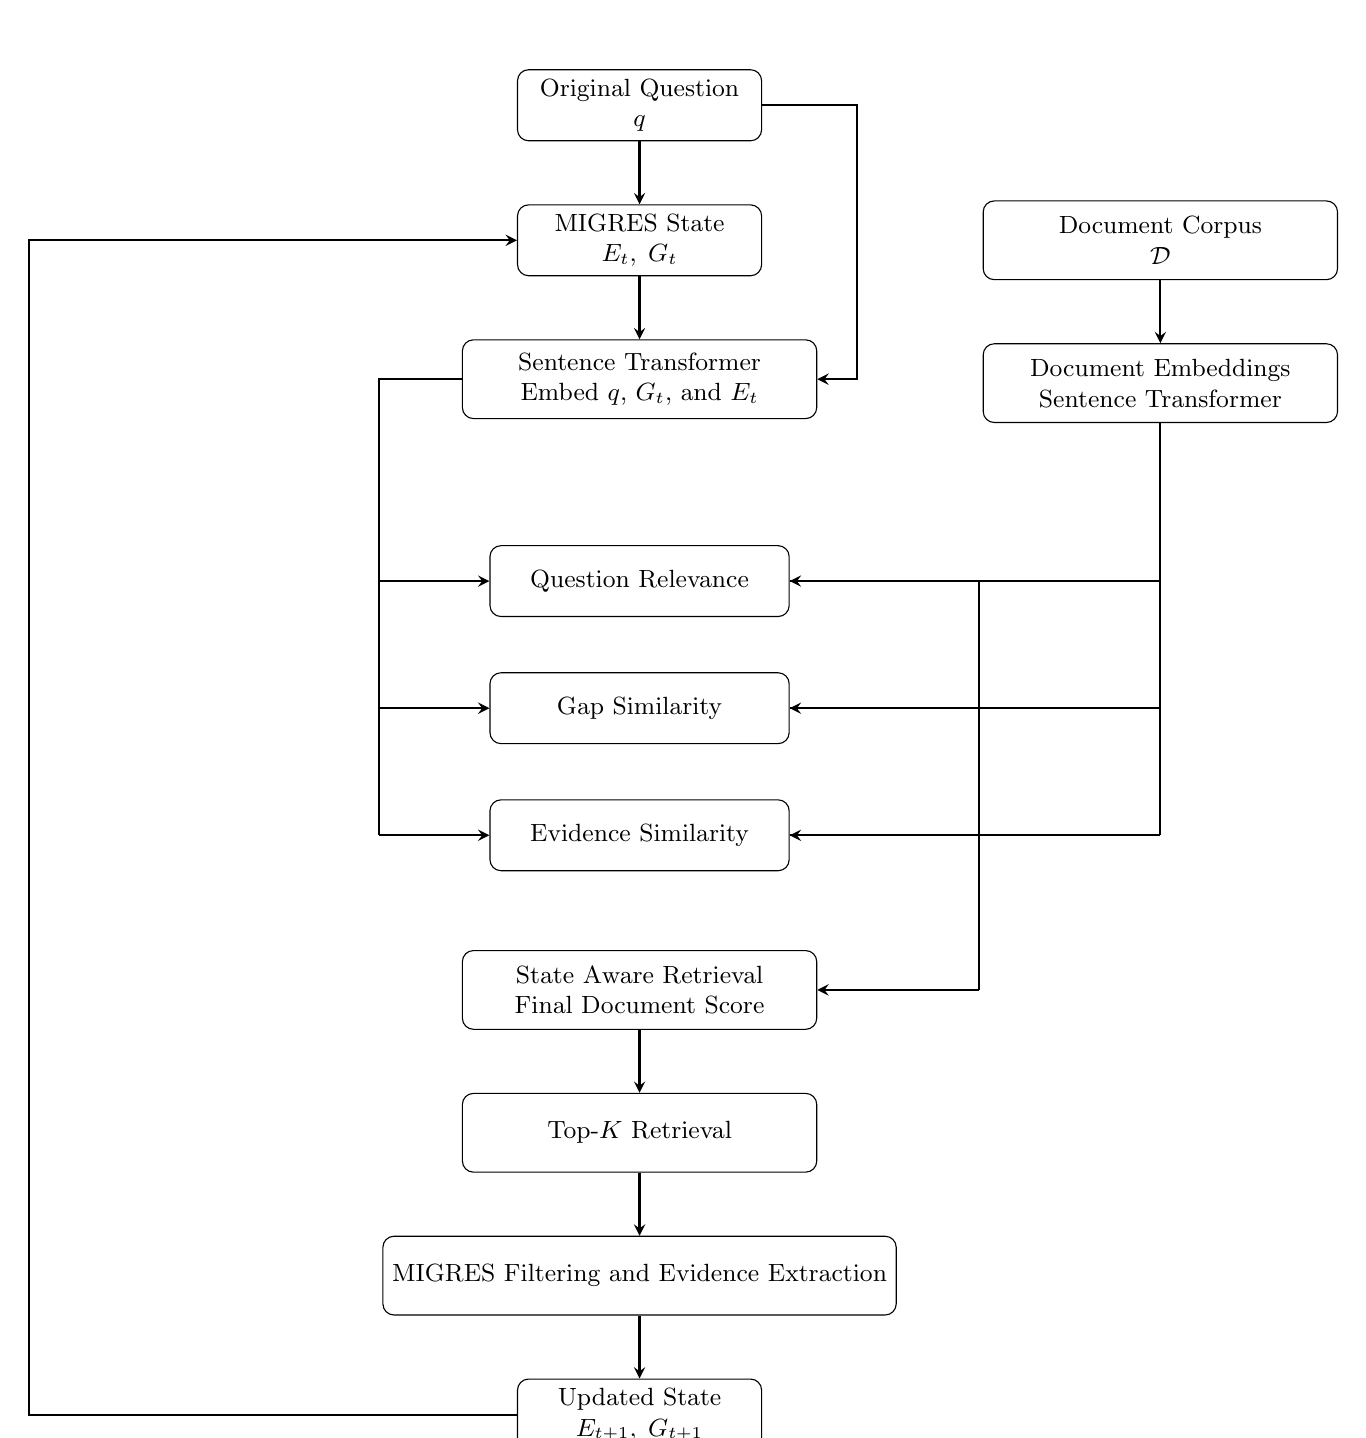
\begin{tikzpicture}[
    node distance=8mm and 18mm,
    box/.style={
        rectangle,
        draw,
        rounded corners,
        align=center,
        minimum width=31mm,
        minimum height=9mm,
        font=\small
    },
    wide/.style={
        rectangle,
        draw,
        rounded corners,
        align=center,
        minimum width=45mm,
        minimum height=10mm,
        font=\small
    },
    simbox/.style={
        rectangle,
        draw,
        rounded corners,
        align=center,
        minimum width=38mm,
        minimum height=9mm,
        font=\small
    },
    arrow/.style={
        ->,
        >=stealth,
        thick
    },
    line/.style={
        thick
    }
]

% ------------------------------------------------------------
% Top level
% ------------------------------------------------------------

\node[box] (q)
    {Original Question\\$q$};

\node[box,below=of q] (state)
    {MIGRES State\\$E_t,\;G_t$};
\node[wide,right=28mm of state] (docs)
    {Document Corpus\\$\mathcal{D}$};

\node[wide,below=of docs] (docembed)
    {Document Embeddings\\
     Sentence Transformer};

\node[wide,below=of state] (stateembed)
    {Sentence Transformer\\Embed $q$, $G_t$, and $E_t$};

% ------------------------------------------------------------
% Similarity layer
% ------------------------------------------------------------

\node[simbox,below=16mm of stateembed] (rel)
    {Question Relevance};

\node[simbox,below=7mm of rel] (gap)
    {Gap Similarity};

\node[simbox,below=7mm of gap] (nov)
    {Evidence Similarity};

% ------------------------------------------------------------
% Scoring and retrieval
% ------------------------------------------------------------

\node[wide,below=10mm of nov] (score)
    {State Aware Retrieval\\Final Document Score};

\node[wide,below=of score] (topk)
    {Top-$K$ Retrieval};

\node[wide,below=of topk] (migres)
    {MIGRES Filtering and Evidence Extraction};

\node[box,below=of migres] (update)
    {Updated State\\$E_{t+1},\;G_{t+1}$};

% ------------------------------------------------------------
% Main flow
% ------------------------------------------------------------

\draw[arrow] (q) -- (state);

\draw[arrow] (state) -- (stateembed);

% Question also goes to the embedding stage
\draw[arrow]
    (q.east)
    -- ++(12mm,0)
    |- (stateembed.east);

% Document corpus
\draw[arrow] (docs) -- (docembed);

% ------------------------------------------------------------
% State embedding bus
% ------------------------------------------------------------

\coordinate (sbusTop) at ([xshift=-14mm]rel.west);
\coordinate (sbusBottom) at ([xshift=-14mm]nov.west);

\draw[line]
    (stateembed.west)
    -| (sbusTop)
    -- (sbusBottom);

\draw[arrow]
    (sbusTop)
    -- (rel.west);

\draw[arrow]
    (sbusTop |- gap.west)
    -- (gap.west);

\draw[arrow]
    (sbusTop |- nov.west)
    -- (nov.west);

% ------------------------------------------------------------
% Document embedding bus
% ------------------------------------------------------------

\coordinate (dbusTop) at ([xshift=47mm]rel.east);
\coordinate (dbusBottom) at ([xshift=47mm]nov.east);

\draw[line]
    (docembed.south)
    -| (dbusTop)
    -- (dbusBottom);

\draw[arrow]
    (dbusTop)
    -- (rel.east);

\draw[arrow]
    (dbusTop |- gap.east)
    -- (gap.east);

\draw[arrow]
    (dbusTop |- nov.east)
    -- (nov.east);

% ------------------------------------------------------------
% Similarity outputs to score
% ------------------------------------------------------------

\coordinate (scorebus) at ([xshift=24mm]nov.east);

\draw[line]
    (rel.east)
    -- (scorebus |- rel.east);

\draw[line]
    (gap.east)
    -- (scorebus |- gap.east);

\draw[line]
    (nov.east)
    -- (scorebus |- nov.east);

\draw[line]
    (scorebus |- rel.east)
    -- (scorebus |- score.east);

\draw[arrow]
    (scorebus |- score.east)
    -- (score.east);

% ------------------------------------------------------------
% Retrieval and feedback
% ------------------------------------------------------------

\draw[arrow] (score) -- (topk);

\draw[arrow] (topk) -- (migres);

\draw[arrow] (migres) -- (update);

\draw[arrow]
    (update.west)
    -- ++(-62mm,0)
    |- (state.west);

\end{tikzpicture}

\caption{Architecture of State Aware Retrieval}
\label{fig:sar-architecture}
\end{figure}

\clearpage

% ------------------------------------------------------------
\subsection{Operational Flow}
% ------------------------------------------------------------

The operational flow describes how the proposed system performs retrieval at each iteration. MIGRES provides the current question, evidence, and information gaps. These inputs are embedded and compared with the document corpus. State Aware Retrieval then scores and selects the top-$K$ documents, which are passed to MIGRES for filtering, evidence extraction, and state update. The updated state is used in the next iteration.

\begin{figure}[H]
\centering
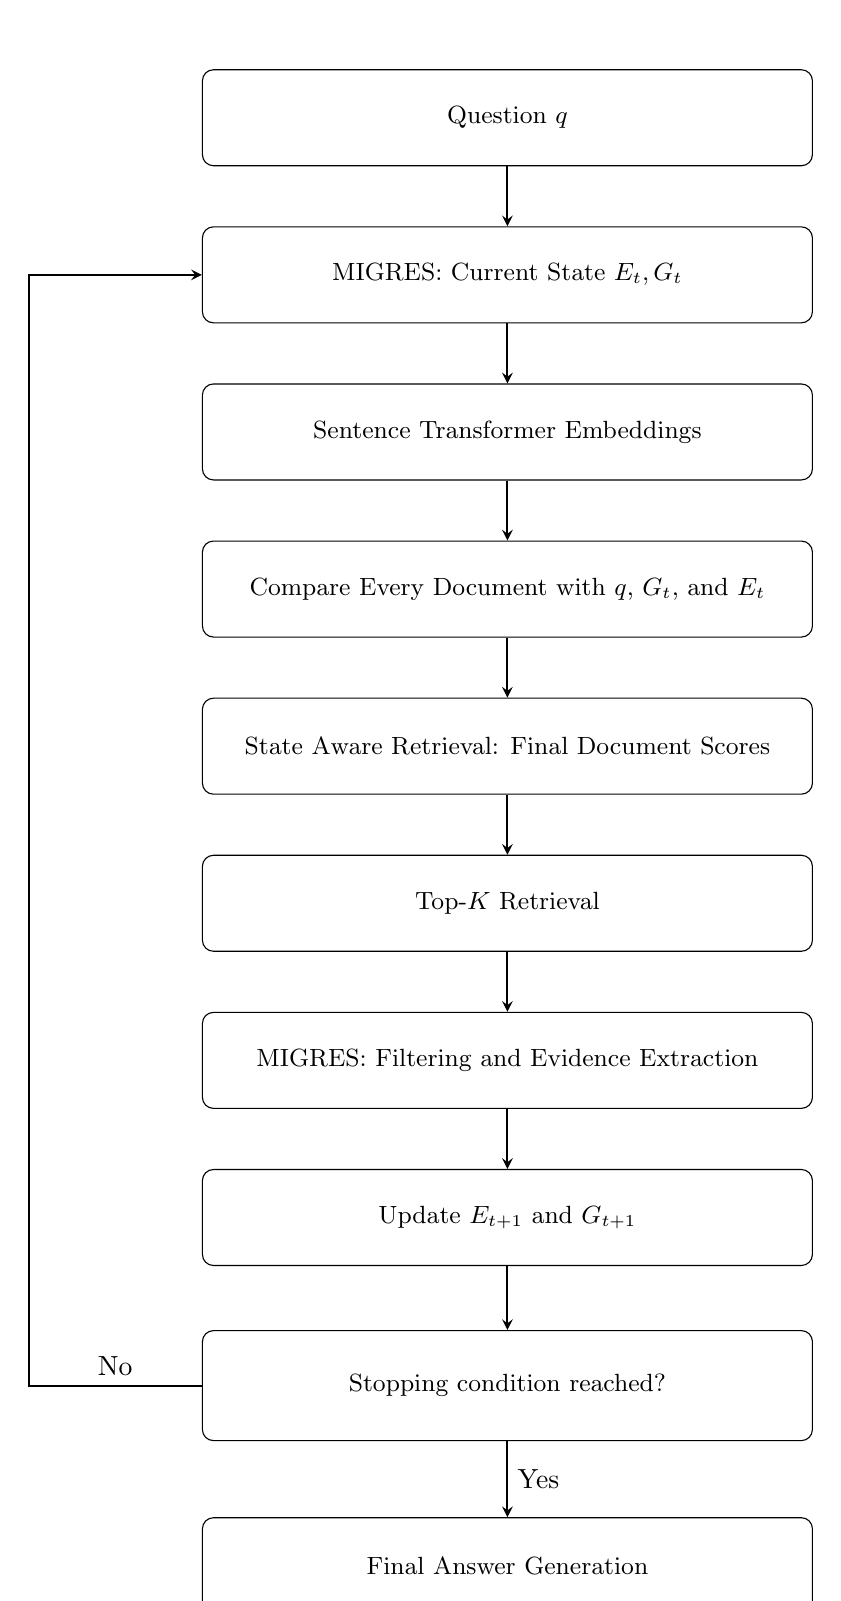
\begin{tikzpicture}[
    node distance=0.30in,
    flowbox/.style={draw,rounded corners,align=center,minimum width=3.05in,minimum height=0.48in,font=\small},
    decision/.style={draw,rounded corners,align=center,minimum width=3.05in,minimum height=0.55in,font=\small},
    arrow/.style={->,>=stealth,line width=0.7pt}
]
\node[flowbox] (question) {Question $q$};
\node[flowbox,below=of question] (state) {MIGRES: Current State $E_t,G_t$};
\node[flowbox,below=of state] (embed) {Sentence Transformer Embeddings};
\node[flowbox,below=of embed] (compare) {Compare Every Document with $q$, $G_t$, and $E_t$};
\node[flowbox,below=of compare] (score) {State Aware Retrieval: Final Document Scores};
\node[flowbox,below=of score] (topk) {Top-$K$ Retrieval};
\node[flowbox,below=of topk] (extract) {MIGRES: Filtering and Evidence Extraction};
\node[flowbox,below=of extract] (update) {Update $E_{t+1}$ and $G_{t+1}$};
\node[decision,below=0.32in of update] (stop) {Stopping condition reached?};
\node[flowbox,below=0.38in of stop] (answer) {Final Answer Generation};

\draw[arrow] (question) -- (state);
\draw[arrow] (state) -- (embed);
\draw[arrow] (embed) -- (compare);
\draw[arrow] (compare) -- (score);
\draw[arrow] (score) -- (topk);
\draw[arrow] (topk) -- (extract);
\draw[arrow] (extract) -- (update);
\draw[arrow] (update) -- (stop);
\draw[arrow] (stop) -- node[right]{Yes} (answer);
\draw[arrow] (stop.west) -- ++(-22mm,0) node[above,midway]{No} |- (state.west);
\end{tikzpicture}
\caption{Operational Flow of State Aware Retrieval}
\label{fig:sar-flow}
\end{figure}

\clearpage

% ------------------------------------------------------------
\section{Mathematical Formulation}
\label{sec:math}

At iteration $t$, the retrieval state contains the question $q$, the collected evidence $E_t$, the current information gap $G_t$, and the complete corpus $\mathcal{D}$. The retrieval method uses this state to assign one final score to every document in the corpus.

\subsection{Notation}

Let
\[
E_t=\{e_1,e_2,\ldots,e_n\}
\]
be the evidence collected before iteration $t$, and let
\[
G_t=\{g_1,g_2,\ldots,g_m\}
\]
be the information gaps identified by MIGRES. The searchable document corpus is:
\[
\mathcal{D}=\{d_1,d_2,\ldots,d_N\}.
\]

The current retrieval state is represented as:
\[
\boxed{(q,E_t,G_t,\mathcal{D})}.
\]

The first retrieval iteration is indexed $t=0$, and at this point there is no evidence and no gap, so $E_0=\emptyset$ and $G_0=\emptyset$. In the implementation, $E_t$ is the list of useful information that MIGRES has extracted so far, and $G_t$ is the list of sub-queries that MIGRES creates for the information that is still missing.

\subsection{Corpus Embedding}

Before retrieval begins, all documents in the corpus are encoded using the selected Sentence Transformer model. The resulting document embeddings are stored and reused during retrieval:
\[
\phi(d) \leftarrow \text{Sentence Transformer}(d).
\]

At the end of each retrieval iteration, the system checks whether any documents in the corpus are new or changed. A new document is converted into a vector with the same model and added to the stored vectors. A changed document is converted again and its old vector is replaced. Documents that have not changed are left as they are, so nothing is converted twice.

\subsection{State Embedding}

At each iteration, the question, current gaps, and collected evidence are encoded using the same Sentence Transformer:
\[
\phi(q),\qquad \phi(g_i),\qquad \phi(e_j).
\]

This places the question, gaps, evidence, and documents in the same semantic space.

\subsection{Sentence Similarity}

The semantic similarity between two text items $x$ and $y$ is measured using cosine similarity, which is commonly used to compare sentence embeddings \cite{reimers2019sentence}:
\[
\operatorname{cos}(x,y)=
\frac{\phi(x)^T\phi(y)}{\|\phi(x)\|_2\|\phi(y)\|_2}.
\]

For the proposed scoring method, the value is normalized to the range $[0,1]$ using:
\[
\boxed{
 s(x,y)=\frac{1+\operatorname{cos}(x,y)}{2}
}
\tag{1}
\]

A higher value means that the two representations are more semantically similar.

\subsection{Question Relevance}

Question relevance measures how close a document is to the original question $q$. It uses the similarity $s(d,q)$ from Eq.~1, which is a value between 0 and 1:
\[
\boxed{R(d,q)=s(d,q)}
\tag{2}
\]

Here $R(d,q)$ is the question relevance score of document $d$. A higher value means the document is more related to the main question. This signal keeps the retrieved documents on the topic of the question. It is the same kind of signal that dense retrievers use to rank passages for a question \cite{karpukhin2020dpr}.

\subsection{Gap Coverage}

At iteration $t$, MIGRES provides $m$ information gaps $G_t=\{g_1,\dots,g_m\}$, where each $g_i$ is a sub-query for one piece of missing information. First, the document $d$ is compared with each gap separately:
\[
\boxed{c(d,g_i)=s(d,g_i)}
\tag{3}
\]

Here $c(d,g_i)$ is the score of document $d$ for the single gap $g_i$. A high value means the document is close to that missing piece.

Next, the scores for all gaps are averaged into one value:
\[
\boxed{
C(d,G_t)=\frac{1}{m}\sum_{i=1}^{m}c(d,g_i)
}
\tag{4}
\]

A higher $C(d,G_t)$ means the document is closer to the information that is still missing. At the first iteration there are no gaps ($G_0=\emptyset$), so the gap coverage is set to $C(d,G_0)=0$. If no gap is left after an iteration, MIGRES can stop the retrieval.

\subsection{Evidence Novelty}

Evidence novelty measures how much new information a document brings compared with the evidence $E_t=\{e_1,\dots,e_n\}$ already collected by MIGRES. First, the document $d$ is compared with every evidence item $e_j$ using $s(d,e_j)$, and the highest value is kept. This highest value shows how much the document repeats its closest piece of evidence. The novelty score is then one minus this value:
\[
\boxed{
N(d,E_t)=1-\max_{e_j\in E_t}s(d,e_j)
}
\tag{5}
\]

A document that is very similar to some collected evidence has a high maximum similarity, so it receives a low novelty value. A document that is not similar to any collected evidence receives a high novelty value. This follows the idea of diversity-aware ranking, where a document is penalized for being similar to items that were already selected \cite{carbonell1998mmr,agrawal2009diversifying}, but here the comparison is made with the collected evidence. At the first iteration no evidence has been collected, so every document is treated as fully new:
\[
\boxed{N(d,E_0)=1.}
\tag{6}
\]

\subsection{State Aware Document Score}

The three signals are combined into one final score for every document. Each signal is multiplied by a weight and the results are added:
\[
\boxed{
S_t(d\mid q,E_t,G_t)=
\alpha R(d,q)+\beta C(d,G_t)+\gamma N(d,E_t)
}
\tag{7}
\]

The weights are never negative and together they add up to one:
\[
\boxed{
\alpha,\beta,\gamma\geq0,
\qquad
\alpha+\beta+\gamma=1.
}
\tag{8}
\]

Here, $\alpha$ controls how much question relevance matters, $\beta$ controls how much gap coverage matters, and $\gamma$ controls how much novelty matters. The weights are needed because the three signals work in different directions. Relevance and gap coverage reward documents that are similar to the question or the missing information, while novelty rewards documents that are different from the collected evidence. An unrelated document is very different from the evidence and can therefore receive a high novelty score. The weights balance the signals so that novelty does not outweigh relevance. At the first iteration, $C=0$ and $N=1$ for every document, so only $R(d,q)$ changes the order of the documents.

\subsection{Top-$K$ Retrieval}

After the final score $S_t$ is calculated for every document in the corpus $\mathcal{D}$, the documents are ranked from the highest score to the lowest. The $K$ documents with the highest scores form the retrieval result:
\[
\boxed{
T_t=\operatorname{TopK}_{d\in\mathcal{D}} S_t(d\mid q,E_t,G_t)
}
\tag{9}
\]

Here $T_t$ is the set of documents selected at iteration $t$, and $K$ is the number of documents returned. No fixed similarity threshold is used before the Top-$K$ selection, so the $K$ best-scored documents are always returned.

\subsection{Iterative State Update}

The selected documents $T_t$ are passed to MIGRES for filtering and information extraction. The useful extracted information is added to the evidence state, and MIGRES identifies the remaining gap for the next iteration:
\[
\boxed{
(q,E_t,G_t,\mathcal{D})
\rightarrow
T_t
\rightarrow
(E_{t+1},G_{t+1})
\rightarrow
T_{t+1}
}
\tag{10}
\]

The process continues until MIGRES determines that enough information has been collected or the MIGRES iteration limit (5 by default) is reached.
\clearpage

% ------------------------------------------------------------
\section{State Aware Retrieval Configurations}

Table~\ref{tab:sar-settings} lists the main configuration of the proposed State Aware Retrieval system. It specifies the models, similarity method, retrieval space, document embedding setup, and other tools used in the project.

\begin{table}[H]
\centering
\caption{State Aware Retrieval Configuration}
\label{tab:sar-settings}
\renewcommand{\arraystretch}{1.2}
\begin{tabular}{|p{1.75in}|p{1.35in}|p{3.0in}|}
\hline
\textbf{Setting} & \textbf{Value} & \textbf{Purpose} \\ \hline
Embedding model & multi-qa-mpnet-\allowbreak base-cos-v1 & Creates common semantic representations for questions, documents, gaps, and evidence. \\ \hline
Similarity function & Cosine similarity & Measures semantic similarity between embedding vectors. \\ \hline
Retrieval space & Complete document corpus $\mathcal{D}$ & Every document is considered during State Aware Retrieval. \\ \hline
Document embeddings & Precomputed and maintained & Stored once and updated when new or changed documents appear. \\ \hline
Framework & MIGRES & Provides the iterative evidence and information-gap state. \\ \hline
LLM API & gemini-3.5-flash-lite & Language model used by MIGRES, called through the Gemini API in the same request format as the original MIGRES code. \\ \hline
\end{tabular}
\end{table}

The weights $\alpha$, $\beta$, and $\gamma$ (Table~\ref{tab:sar-hyperparameters}) follow the constraint in Eq.~8 and are fixed before the final test evaluation. The value of $K$ (50) follows the candidate pool size of the original MIGRES retriever. The iteration limit (5) and the stopping rule are also taken from MIGRES, so all three are the same for SAR and every baseline. SAR and every baseline also use the same language model and call settings, with the default temperature of the provider.

\begin{table}[H]
\centering
\caption{State Aware Retrieval Hyperparameters}
\label{tab:sar-hyperparameters}
\renewcommand{\arraystretch}{1.2}
\begin{tabular}{|p{1.3in}|p{2.0in}|p{2.8in}|}
\hline
\textbf{Hyperparameter} & \textbf{Role} & \textbf{Selection} \\ \hline
$\alpha$ & Question relevance weight & Bayesian optimization on validation data. \\ \hline
$\beta$ & Gap coverage weight & Bayesian optimization on validation data. \\ \hline
$\gamma$ & Evidence novelty weight & Bayesian optimization on validation data. \\ \hline
\end{tabular}
\end{table}
\clearpage
% ------------------------------------------------------------
\section{Datasets and Model}
% ------------------------------------------------------------

\subsection{Datasets}

The evaluation uses three question-answering datasets from the MIGRES setting. They cover multi-hop reasoning and open-domain question answering.

\subsubsection{HotpotQA}

HotpotQA \cite{yang2018hotpotqa} has about 113,000 crowd-written questions over Wikipedia. Each question needs facts from two or more paragraphs, either as a \textit{bridge} (one fact leads to the next) or a \textit{comparison}. The supporting sentences are marked, so the retrieved evidence can be checked. In the distractor setting, each question has 10 paragraphs (2 correct, 8 distractors), and in the full-wiki setting the evidence is searched from all of Wikipedia.

Every question is stored as one record with fields such as the following:

\begin{center}
\begin{tabular}{|p{1.4in}|p{4.6in}|}
\hline
\textbf{Field} & \textbf{Example} \\ \hline
\texttt{question} & Were Scott Derrickson and Ed Wood of the same nationality? \\ \hline
\texttt{answer} & yes \\ \hline
\texttt{supporting\_facts} & Page titles and sentence numbers of the proof sentences \\ \hline
\texttt{context} & The Wikipedia paragraphs given for the question \\ \hline
\texttt{type} & comparison (or bridge) \\ \hline
\texttt{level} & easy, medium, or hard \\ \hline
\end{tabular}
\end{center}

\subsubsection{MuSiQue}

MuSiQue \cite{trivedi2022musique} has about 25,000 questions that need two to four reasoning steps, where the answer to one step is used in the next. The questions are built by joining simple one-step questions, and each comes with 20 Wikipedia paragraphs, most of them distractors. The design prevents a model from answering through shortcuts.

Every question is stored as one record with fields such as the following:

\begin{center}
\begin{tabular}{|p{2.2in}|p{3.8in}|}
\hline
\textbf{Field} & \textbf{Content} \\ \hline
\texttt{question} & The full multi-step question \\ \hline
\texttt{question\_\allowbreak decomposition} & The smaller one-step questions, in order \\ \hline
\texttt{paragraphs} & The 20 paragraphs, each with a title, text, and a mark showing if it is a correct (supporting) paragraph \\ \hline
\texttt{answer} & The short final answer \\ \hline
\texttt{answer\_aliases} & Other accepted ways to write the answer \\ \hline
\texttt{answerable} & True or false \\ \hline
\end{tabular}
\end{center}

\subsubsection{Natural Questions}

Natural Questions \cite{kwiatkowski2019natural} contains real, short queries typed into Google, with Wikipedia pages as the source. Annotators marked the answer, or marked that the page has none. Most questions need only one passage, so it tests standard open-domain question answering. It has more than 300,000 training questions.

Every question is stored as one record with fields such as the following:

\begin{center}
\begin{tabular}{|p{1.6in}|p{4.4in}|}
\hline
\textbf{Field} & \textbf{Content} \\ \hline
\texttt{question\_text} & The search query, e.g., who sings what a wonderful world \\ \hline
\texttt{document} & The Wikipedia page found for the question \\ \hline
\texttt{long\_answer} & The paragraph that contains the answer, or empty if none \\ \hline
\texttt{short\_answers} & The exact answer words from that paragraph, or empty \\ \hline
\texttt{yes\_no\_answer} & Yes, no, or none \\ \hline
\end{tabular}
\end{center}

\subsection{Models}

\begin{table}[H]
\centering
\caption{Models used in SAR, MIGRES, and baseline systems.}
\label{tab:models}
\renewcommand{\arraystretch}{1.25}
\begin{tabular}{|p{5.0cm}|p{8.0cm}|}
\hline
\textbf{Model} & \textbf{Role} \\
\hline
\texttt{sentence-transformers/\allowbreak multi-qa-mpnet-\allowbreak base-cos-v1} (768-d) &
Sentence Transformer \cite{reimers2019sentence,song2020mpnet,st2020mpnet} used for document, question, information-gap, and evidence embeddings in SAR. The same model is used for SAR cosine-similarity scoring and the Sentence Transformer Search baseline. \\
\hline
\texttt{gemini-3.5-flash-lite} &
Language model \cite{gemini2023} used by MIGRES for evidence extraction, information-gap detection, sub-query generation, and final answer generation. The same model and call settings are used across SAR and all baselines. \\
\hline
\texttt{BAAI/bge-reranker-base} &
Cross-encoder reranker \cite{nogueira2019passage,xiao2024cpack} used by MIGRES to filter and rerank retrieved passages after each retrieval step. \\
\hline
\end{tabular}
\end{table}

\clearpage
% ------------------------------------------------------------
\section{Experimental Design}

The experiments evaluate State Aware Retrieval from several perspectives. The study includes hyperparameter selection, comparison with existing retrieval methods, ablation testing, retrieval performance evaluation, iterative state analysis, downstream RAG and robustness evaluation, and computational cost analysis. The validation data are used to tune the scoring weights, and the selected weights are then fixed before the final test evaluation.

% ------------------------------------------------------------
\subsection{Hyperparameter Selection}

SAR scores each document using three signals: question relevance, gap coverage, and evidence novelty. The weights $\alpha$, $\beta$, and $\gamma$ (Table~\ref{tab:sar-hyperparameters}) set how much each signal counts.

The best balance between the three signals is not known in advance. The weights are non-negative and sum to one (Eq.~8), so only two values are free. They are selected before all other experiments using Bayesian optimization \cite{snoek2012practical}, a search method that learns from earlier trials and chooses the next weights that look most promising. It suits this task because each trial needs a full MIGRES run, so only a few trials are affordable.

\begin{itemize}[leftmargin=0.25in,itemsep=0.06in,parsep=0pt]
\item \textbf{Trials:} 10 in total, where the first 3 use random weights and the next 7 are proposed by the optimizer.
\item \textbf{One trial:} SAR is run within MIGRES with the candidate weights on 8 validation questions from each of the three datasets, and the trial is scored by the mean Recall@$K$.
\item \textbf{Seed:} one fixed random seed is used, so that the search can be repeated.
\item \textbf{Result:} the weights with the best score are selected, fixed, and used in all later experiments.
\end{itemize}

Only validation data are used, so the evaluation questions do not influence the weights.

% ------------------------------------------------------------
\subsection{Baseline Comparison}

State Aware Retrieval is compared with four established retrieval methods, listed in Table~\ref{tab:baseline-comparison}. All methods use the same document corpus, evaluation questions, and retrieval depth. Each baseline replaces the SAR retrieval step inside the same MIGRES loop. When MIGRES sends several queries, the highest score of each document is kept before the common Top-$K$ selection and filtering steps. Only SAR uses the Sentence Transformer model; the baselines use their own representations. Other retrieval families, such as learned sparse retrieval \cite{formal2021splade} and late interaction \cite{khattab2020colbert,santhanam2022colbertv2}, are reviewed in Chapter~2 but are not used as baselines.

\begin{table}[H]
\centering
\caption{Information Retrieval Baseline Comparison}
\label{tab:baseline-comparison}
\renewcommand{\arraystretch}{1.2}
\begin{tabular}{|p{1.55in}|p{1.40in}|p{3.10in}|}
\hline
\textbf{System} & \textbf{Type} & \textbf{Main Retrieval Basis} \\ \hline
BM25 & Sparse lexical &
Term frequency, inverse document frequency, and document length
\cite{robertson2009bm25} \\ \hline

DPR & Dense &
Question and passage embeddings learned with a dual encoder
\cite{karpukhin2020dpr} \\ \hline

Contriever & Dense &
Unsupervised dense representations for semantic retrieval
\cite{izacard2022contriever} \\ \hline

MMR & Lexical, diversity-aware &
BM25 candidates re-ranked by maximal marginal relevance
\cite{carbonell1998mmr} \\ \hline

State Aware Retrieval & multi-signal dense retrieval &
Question relevance, gap coverage, and evidence novelty \\ \hline
\end{tabular}
\end{table}
% ------------------------------------------------------------
\subsection{Ablation Study}

The ablation study measures the contribution of each signal used by State Aware Retrieval. The full SAR configuration is compared with versions in which individual signals or the weight tuning are removed.

\begin{itemize}[leftmargin=0.25in,itemsep=0.06in,parsep=0pt]
\item \textbf{SAR-Full:} question relevance, gap coverage, and evidence novelty, with the weights selected by Bayesian optimization.
\item \textbf{SAR-Without-Relevance:} removes question relevance.
\item \textbf{SAR-Without-Gap:} removes gap coverage.
\item \textbf{SAR-Without-Evidence:} removes evidence novelty.
\item \textbf{SAR-Without-Tuning:} keeps all three signals but does not use the optimized weights. Equal weights $\alpha=\beta=\gamma=\tfrac{1}{3}$ are used instead.
\item \textbf{Question-Only:} uses only the similarity between the document and the original question.
\end{itemize}

% ------------------------------------------------------------
\subsection{Retrieval Performance Evaluation}

The retrieval experiment evaluates the quality of the documents selected by State Aware Retrieval. The SAR configuration fixed after validation is compared with the baselines on the raw ranking of each retriever, before the MIGRES filter is applied. For each question, the Top-$K$ documents are checked against the relevant documents of the dataset using standard ranking metrics \cite{manning2008ir}, and each metric is averaged over all evaluation questions.

\begin{itemize}[leftmargin=0.25in,itemsep=0.06in,parsep=0pt]
\item \textbf{Recall@$K$:} the share of the relevant documents that appear in the Top-$K$. It shows how much of the needed evidence is retrieved.
\item \textbf{Precision@$K$:} the share of the Top-$K$ documents that are relevant. It shows how clean the retrieved set is.
\item \textbf{Hit@$K$:} whether at least one relevant document appears in the Top-$K$ (1 if yes, 0 if no).
\item \textbf{Mean Reciprocal Rank (MRR):} the average of one divided by the rank of the first relevant document, taken as 0 if none is retrieved. A higher value means that a relevant document appears earlier.
\item \textbf{nDCG@$K$:} how good the ranking order is. Relevant documents placed higher count more, and the score is compared with the best possible order \cite{jarvelin2002cumulated}.
\end{itemize}

% ------------------------------------------------------------
\subsection{Iterative State Analysis}

State Aware Retrieval is intended to change its retrieval behavior as the evidence and information gaps change. This experiment studies the retrieved documents across successive iterations. In the results, iterations are counted from 1, so the first iteration corresponds to $t=0$ in Section~\ref{sec:math}, and the comparison between consecutive iterations starts from the second iteration.

\begin{itemize}[leftmargin=0.25in,itemsep=0.06in,parsep=0pt]
\item \textbf{Cumulative recall:} the share of the relevant documents found up to the current iteration.
\item \textbf{Marginal recall gain:} the additional relevant documents found at the current iteration compared with the previous iterations.
\item \textbf{New document rate:} the share of the documents retrieved at the current iteration that were not retrieved in any earlier iteration.
\item \textbf{Retrieval overlap:} how much the documents retrieved at the current iteration overlap with those of the previous iteration.
\end{itemize}

Together, these measures show whether the changing evidence and gaps lead to different and complementary retrieval results at each iteration.

% ------------------------------------------------------------
\subsection{Downstream RAG and Robustness Evaluation}
\label{sec:downstream}

State Aware Retrieval is evaluated within the MIGRES framework to measure its effect on the final answer. SAR and the baselines use the same MIGRES configuration and language model. The common MIGRES filter is applied after every retriever, so the answer metrics reflect the filtered evidence. The number of documents kept by the filter is recorded separately, because the filter can change which of the retrieved documents reach the answer step.

\subsubsection{Answer Evaluation}

Answer quality is measured with the official metrics of each dataset where available. Questions without gold answers are excluded.

\begin{itemize}[leftmargin=0.25in,itemsep=0.06in,parsep=0pt]
\item \textbf{Exact Match (EM):} the share of answers that exactly match a gold answer.
\item \textbf{Accuracy:} the share of correct answers, checked by normalized exact match against the gold answers and their aliases. No substring match or language-model judge is used.
\item \textbf{Token-level F1:} the word overlap between the predicted answer and the gold answer, which gives partial credit to partly correct answers \cite{rajpurkar2016squad}.
\end{itemize}

\subsubsection{RGB Robustness}

The Retrieval-Augmented Generation Benchmark (RGB) tests robustness in four settings \cite{chen2024rgb}:

\begin{itemize}[leftmargin=0.25in,itemsep=0.06in,parsep=0pt]
\item \textbf{Noise robustness:} answer accuracy when irrelevant documents are mixed into the retrieved set, at different noise levels.
\item \textbf{Negative rejection:} how often the system correctly refuses to answer when the documents contain no answer.
\item \textbf{Information integration:} answer accuracy on questions that need information from several documents.
\item \textbf{Counterfactual robustness:} how often the system detects wrong information in the documents (error detection) and corrects it (error correction).
\end{itemize}

% ------------------------------------------------------------
\subsection{Computational Cost Analysis}

SAR scores every document in the corpus at each iteration, so it may need more computation than a method that scores only a candidate list. SAR computes exact scores for all documents instead of using an approximate nearest-neighbor index \cite{johnson2017billion}. This experiment measures that extra cost. SAR and the baselines run in the same MIGRES loop with the same corpus, the same $K$, and the same language model settings, so any difference in cost comes from the retrieval method alone.

\begin{itemize}[leftmargin=0.25in,itemsep=0.06in,parsep=0pt]
\item \textbf{Index build time:} the one-time time needed to embed the corpus and store the document vectors.
\item \textbf{Retrieval latency:} the average time taken by the retrieval step per iteration, split into the time to embed the question, gaps, and evidence and the time to score the documents.
\item \textbf{Scoring workload:} the number of documents scored and the number of similarity calculations per question.
\item \textbf{Language model usage:} the number of language model calls and tokens per question.
\end{itemize}

% ------------------------------------------------------------
\section{Chapter Solution Summary}

This chapter presented State Aware Retrieval (SAR) as a direct retrieval
method within the MIGRES framework. SAR uses the current question,
information gaps, and collected evidence to guide document selection
from the complete document corpus.

The documents are represented in a common Sentence Transformer
embedding space. At each iteration, the documents are compared with the
current retrieval state, and the final score is used to select the
Top-$K$ documents. The selected documents are then passed to MIGRES for
filtering, evidence extraction, and state update.

SAR scores the complete corpus directly, with no fixed retrieval threshold. The scoring formulation is defined in Section~\ref{sec:math}, and its weights are selected using validation data. The experiments evaluate the contribution of each state signal, compare SAR with existing retrieval methods, measure retrieval and downstream RAG performance, study its behavior across iterations, and measure its computational cost. The next chapter lists the software and hardware needed to carry out this work.
\label{ch:5:end}

\clearpage

% ============================================================
% CHAPTER 6
% SOFTWARE AND HARDWARE REQUIREMENTS
% ============================================================

\setcounter{table}{0}
\renewcommand{\thetable}{6.\arabic{table}}
\renewcommand{\theHtable}{chapter6.\arabic{table}}

\addcontentsline{toc}{chapter}{6. SOFTWARE AND HARDWARE REQUIREMENTS}

\chaptertitle{6}{SOFTWARE AND HARDWARE REQUIREMENTS}
\label{ch:6}

\justifying

The proposed solution uses a Python-based environment for dataset
preparation, document embedding, State Aware Retrieval, hyperparameter
selection, MIGRES integration, and evaluation. Jupyter Notebook \cite{kluyver2016jupyter} is used
for experiment development and analysis, and LaTeX is used to prepare
this report. The main software and hardware requirements are described
below.

\section*{6.1 Software Requirements}

\begin{table}[H]
\centering
\caption{Software Requirements}
\label{tab:software-requirements}
\renewcommand{\arraystretch}{1.2}
\begin{tabular}{|p{1.65in}|p{1.45in}|p{2.95in}|}
\hline
\textbf{Software / Tool} & \textbf{Version} & \textbf{Purpose} \\ \hline

Python & 3.12.10 &
Main programming environment for data processing, document embedding,
retrieval, and evaluation. \\ \hline

Visual Studio Code & 1.131 &
Experiment development, execution, and result analysis. \\ \hline

PyTorch \cite{paszke2019pytorch} & 2.13.0 &
Tensor computation and neural model execution. \\ \hline

Sentence Transformers \cite{reimers2019sentence} & 5.6.1 &
Generates semantic embeddings for questions, documents, information
gaps, and evidence using
\texttt{multi-qa-mpnet-base-cos-v1}. \\ \hline

Bayesian Optimization \cite{nogueira2014bayesopt} & 3.3.0 &
Selects the State Aware Retrieval scoring hyperparameters using
validation data. \\ \hline

LaTeX & Overleaf &
Preparation of the research document. \\ \hline

Gemini API \cite{gemini2023} & gemini-3.5-flash-lite &
Provides the language model used by MIGRES for information-gap
processing and response generation. \\ \hline

\end{tabular}
\end{table}
\clearpage
\section*{6.3 Hardware Requirements}

The proposed system can be implemented on a standard computer
with internet access. The main hardware requirements are:

\begin{itemize}
    \item \textbf{CPU:} Intel Core i5 (or equivalent) or higher multi-core processor.
    \item \textbf{RAM:} At least 16 GB.
    \item \textbf{Storage:} At least 20 GB of free SSD space.
    \item \textbf{GPU:} CUDA-compatible NVIDIA GPU with at least 8 GB of VRAM.
    \item \textbf{Network:} Stable internet connection for the language model API and pretrained model downloads.
\end{itemize}
\label{ch:6:end}

\clearpage

% ============================================================
% CHAPTER 7
% IMPLEMENTATION
% ============================================================

\setcounter{table}{0}
\renewcommand{\thetable}{7.\arabic{table}}
\renewcommand{\theHtable}{chapter7.\arabic{table}}
\setcounter{figure}{0}
\renewcommand{\thefigure}{7.\arabic{figure}}
\renewcommand{\theHfigure}{chapter7.\arabic{figure}}
\setcounter{chapter}{7}
\setcounter{section}{0}
\setcounter{subsection}{0}

\addcontentsline{toc}{chapter}{7. IMPLEMENTATION}
\chaptertitle{7}{IMPLEMENTATION}
\label{ch:7}
\justifying

% ============================================================
\section{Introduction}
% ============================================================

This chapter describes the implementation of the proposed SAR-based
retrieval system within the MIGRES framework. It first presents the
development environment, including the hardware and software used. It
then explains how the system is organized and integrated, covering the
document corpus and embedding pipeline, the MIGRES module, and the SAR
retrieval module. The SAR algorithm is then given in pseudocode, and the
chapter ends with the workflow used to execute the prepared experiments.

\tikzset{
    implbox/.style={draw,rounded corners=2pt,align=center,text width=2.2cm,minimum height=1.15cm,inner sep=3pt,font=\scriptsize,execute at begin node={\hyphenpenalty=10000\relax}},
    implar/.style={->,>=stealth,line width=0.65pt}
}

% ============================================================
\section{Development Environment}
% ============================================================

\subsection{Hardware Environment}

The experiments are executed using a Google Colab managed runtime with an NVIDIA Tesla T4 GPU. The T4 provides 16~GB of GDDR6 GPU memory and 2,560 CUDA cores. Google Colab provides the CPU, system memory, and temporary runtime storage as part of the managed notebook environment, with the exact allocation depending on the runtime instance. The experiments therefore use the following compute environment.

\begin{table}[H]
\centering
\caption{Hardware Environment}
\label{tab:hardware-environment}
\renewcommand{\arraystretch}{1.15}
\begin{tabular}{|p{2.2in}|p{3.8in}|}
\hline
\textbf{Component} & \textbf{Specification} \\
\hline
Execution Environment & Google Colab managed runtime \\
\hline
GPU & NVIDIA Tesla T4 \\
\hline
GPU Memory & 16~GB GDDR6 \\
\hline
CUDA Cores & 2,560 \\
\hline
CPU & Colab-managed virtual CPU \\
\hline
System Memory & Colab-managed runtime memory \\
\hline
Storage & Temporary runtime storage provided by Colab \\
\hline
Internet & Required for model downloads, dataset access, and language model API calls \\
\hline
\end{tabular}
\end{table}

\subsection{Software Environment}

The implementation is developed in Python using Visual Studio Code, while the experiments are executed through Jupyter notebooks in Google Colab. Similarity computations use NumPy \cite{harris2020numpy}, and the Sentence Transformers library builds on the Hugging Face Transformers library \cite{wolf2020transformers}. The main software components used in the experimental pipeline are summarized in Table~\ref{tab:software-environment}.

\begin{table}[H]
\centering
\caption{Software Environment}
\label{tab:software-environment}
\renewcommand{\arraystretch}{1.15}
\begin{tabular}{|p{2.35in}|p{3.65in}|}
\hline
\textbf{Software / Tool} & \textbf{Purpose} \\
\hline
Python & Core implementation and experiment pipeline \\
\hline
Visual Studio Code & Development and code management \\
\hline
Jupyter Notebook & Execution and analysis of experiments \\
\hline
PyTorch & Model inference and tensor computation \\
\hline
Sentence Transformers & Document and retrieval-state embeddings \\
\hline
Bayesian Optimization & Selection of SAR weighting parameters \\
\hline
MIGRES Framework & Iterative retrieval and evidence processing \\
\hline
Google Gemini API & Language model operations within MIGRES \\
\hline
Local Disk-backed Vector Store & Storage of precomputed document embeddings \\
\hline
YAML Configuration & Management of model, retrieval, and experiment settings \\
\hline
\end{tabular}
\end{table}

% ============================================================
\section{System Implementation}
% ============================================================

The proposed system is implemented by integrating the SAR retrieval method into the existing MIGRES framework. The implementation is organized into three main components that work together during retrieval. The document corpus and embedding module first prepares the searchable corpus by processing the documents, generating their embeddings, and storing the resulting vectors in the vector store. This preparation is completed before the experiments are executed. During retrieval, MIGRES manages the question-answering process and maintains the current retrieval state, while the SAR module uses the query and state information together with the precomputed document vectors to calculate relevance, gap coverage, and evidence novelty and select the Top-$K$ documents. The retrieved documents are then returned to MIGRES for filtering, evidence extraction, and state updating before the next iteration.
\begin{figure}[H]
\centering
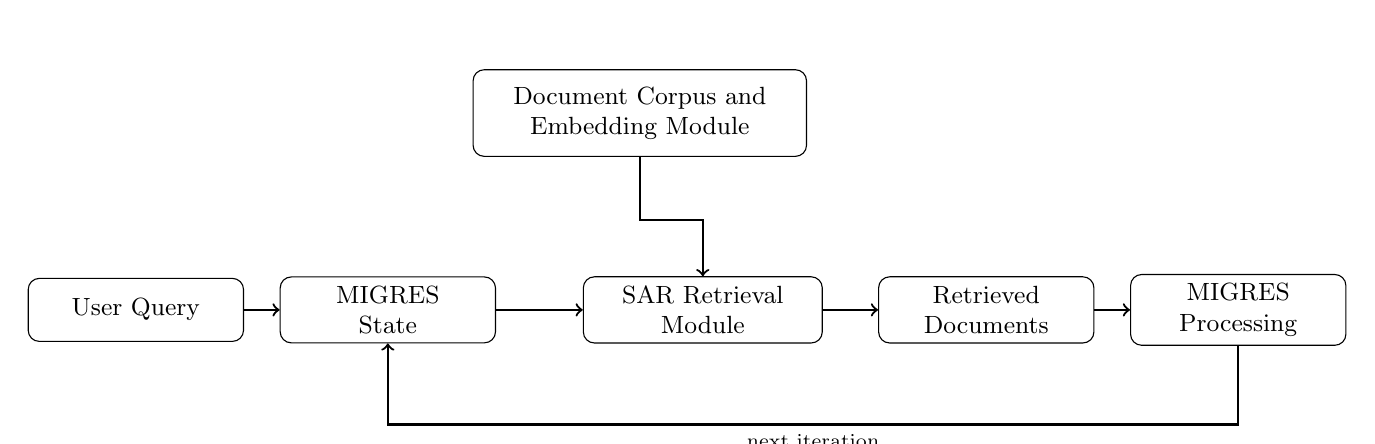
\begin{tikzpicture}[
    box/.style={
        draw,
        rounded corners,
        align=center,
        minimum height=8mm,
        text width=25mm,
        font=\small
    },
    modulebox/.style={
        draw,
        rounded corners,
        align=center,
        minimum height=11mm,
        text width=40mm,
        font=\small
    },
    sarbox/.style={
        draw,
        rounded corners,
        align=center,
        minimum height=8mm,
        text width=28mm,
        font=\small
    },
    arrow/.style={
        ->,
        thick
    }
]

% Document Corpus and Embedding Module
\node[modulebox] (corpus) at (3.2,2.5)
{Document Corpus and\\Embedding Module};

% Retrieval pipeline
\node[box] (query) at (-3.2,0) {User Query};
\node[box] (migres) at (0,0) {MIGRES\\State};
\node[sarbox] (sar) at (4.0,0) {SAR Retrieval\\Module};
\node[box] (docs) at (7.6,0) {Retrieved\\Documents};
\node[box] (processing) at (10.8,0) {MIGRES\\Processing};

\draw[arrow] (query) -- (migres);
\draw[arrow] (migres) -- (sar);
\draw[arrow] (sar) -- (docs);
\draw[arrow] (docs) -- (processing);

% Corpus and embedding module to SAR
\draw[arrow]
    (corpus.south)
    -- ++(0,-8mm)
    -| (sar.north);

% Iteration feedback
\draw[arrow]
    (processing.south)
    |- ++(0,-10mm)
    -| node[pos=0.25,below,font=\scriptsize]{next iteration}
    (migres.south);

\end{tikzpicture}
\caption{Overall System Implementation Flow}
\label{fig:system-implementation}
\end{figure}

\subsection{Document Corpus and Embedding Module}

This module prepares the document collection used by the SAR retriever. Its purpose is to convert the source datasets into a common searchable format and create the vector representations required for retrieval. The module performs four main stages: dataset preparation, passage chunking, document embedding, and vector storage. The resulting vector store is then used by SAR during document scoring and Top-$K$ selection.

The module consists of the following stages:

\begin{figure}[H]
\centering
\resizebox{\textwidth}{!}{%
\begin{tikzpicture}
\node[implbox] (c) at (0,0) {Corpus};
\node[implbox] (p) at (3.2,0) {Processing and Chunking};
\node[implbox] (stm) at (6.4,0) {Sentence Transformer};
\node[implbox] (de) at (9.6,0) {Document Embeddings};
\node[implbox] (vs) at (12.8,0) {Vector Store};
\draw[implar] (c)--(p); \draw[implar] (p)--(stm); \draw[implar] (stm)--(de); \draw[implar] (de)--(vs);
\end{tikzpicture}}
\caption{Corpus Preparation and Embedding Pipeline}
\label{fig:impl-corpus-flow}
\end{figure}

\subsection{MIGRES Module}

MIGRES is the base framework that manages the iterative question-answering process. It maintains the information required at each iteration and controls how retrieved documents are processed until the question can be answered or the stopping condition is reached.

In this project, MIGRES provides the main execution flow, while SAR is integrated as the retrieval method within that flow. The MIGRES implementation can be viewed through two main parts: the retrieval state maintained during each iteration and the processing stage that handles the retrieved documents and updates this state.

The MIGRES state contains the original question $q$, the evidence collected up to iteration $t$, denoted by $E_t$, and the remaining information gaps $G_t$. This state is provided to the retrieval stage for each iteration. After retrieval, MIGRES processes the returned documents through filtering and evidence extraction. It then checks whether sufficient information is available. If further information is required, new queries are generated, the state is updated, and the next retrieval iteration begins.

\begin{figure}[H]
\centering

\resizebox{0.98\textwidth}{!}{%
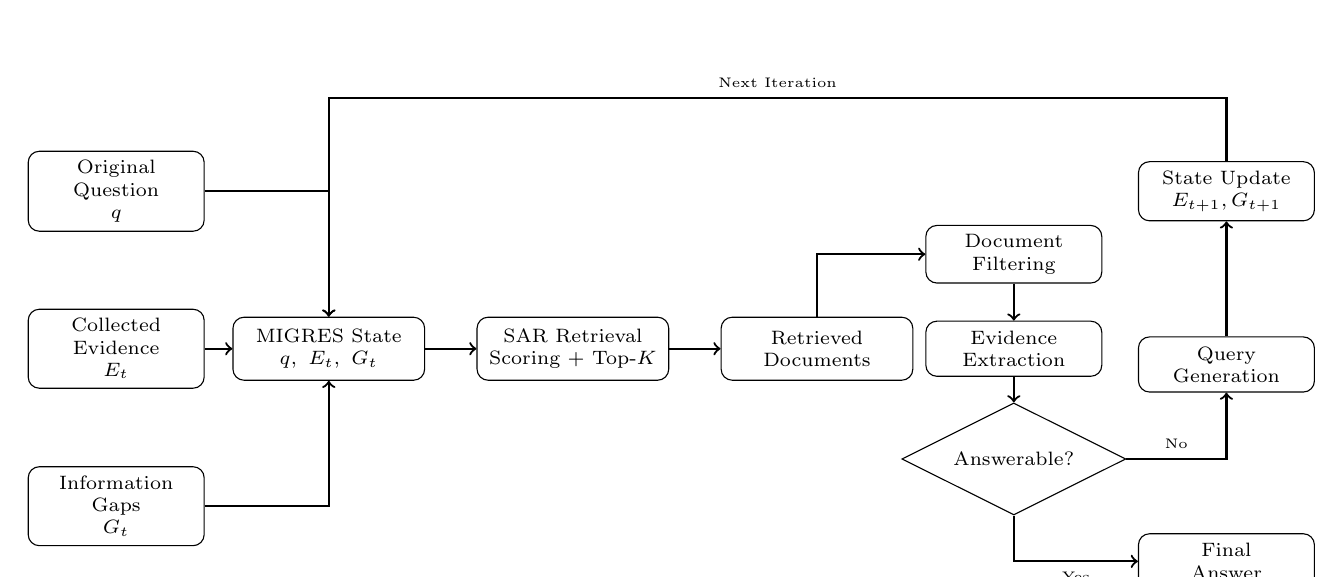
\begin{tikzpicture}[
    box/.style={
        draw,
        rounded corners,
        align=center,
        minimum height=8mm,
        text width=22mm,
        font=\scriptsize
    },
    smallbox/.style={
        draw,
        rounded corners,
        align=center,
        minimum height=7mm,
        text width=20mm,
        font=\scriptsize
    },
    decision/.style={
        diamond,
        draw,
        align=center,
        aspect=2,
        text width=18mm,
        font=\scriptsize
    },
    arrow/.style={
        ->,
        thick
    }
]

% ---------------- MIGRES STATE ----------------

\node[smallbox] (query) at (0,2)
{Original Question\\$q$};

\node[smallbox] (evidence) at (0,0)
{Collected Evidence\\$E_t$};

\node[smallbox] (gaps) at (0,-2)
{Information Gaps\\$G_t$};

\node[box] (state) at (2.7,0)
{MIGRES State\\$q,\ E_t,\ G_t$};

\draw[arrow] (query.east) -| (state.north);
\draw[arrow] (evidence.east) -- (state.west);
\draw[arrow] (gaps.east) -| (state.south);

% ---------------- SAR ----------------

\node[box] (sar) at (5.8,0)
{SAR Retrieval\\Scoring + Top-$K$};

\draw[arrow] (state) -- (sar);

% ---------------- DOCUMENTS ----------------

\node[box] (docs) at (8.9,0)
{Retrieved\\Documents};

\draw[arrow] (sar) -- (docs);

% ---------------- MIGRES PROCESSING ----------------

\node[smallbox] (filter) at (11.4,1.2)
{Document\\Filtering};

\node[smallbox] (extract) at (11.4,0)
{Evidence\\Extraction};

\node[decision] (check) at (11.4,-1.4)
{Answerable?};

\draw[arrow] (docs) |- (filter);
\draw[arrow] (filter) -- (extract);
\draw[arrow] (extract) -- (check);

% ---------------- DECISION ----------------

\node[smallbox] (answer) at (14.1,-2.7)
{Final\\Answer};

\node[smallbox] (generate) at (14.1,-0.2)
{Query\\Generation};

\node[smallbox] (update) at (14.1,2.0)
{State Update\\$E_{t+1},G_{t+1}$};

% Yes path
\draw[arrow]
    (check.south)
    |- node[pos=0.75,below,font=\tiny]{Yes}
    (answer.west);

% No path
\draw[arrow]
    (check.east)
    -| node[pos=0.25,above,font=\tiny]{No}
    (generate.south);

\draw[arrow] (generate) -- (update);

% Next iteration
\draw[arrow]
    (update.north)
    |- ++(0,0.8)
    -| node[pos=0.25,above,font=\tiny]{Next Iteration}
    (state.north);

\end{tikzpicture}%
}

\caption{MIGRES State and Processing Flow with SAR Integration}
\label{fig:migres-state-processing}
\end{figure}

\subsection{SAR Module}

State-Aware Retrieval (SAR) is the retrieval method proposed in this project. It selects documents based on the current retrieval state rather than using only the original question. The state consists of the question $q$, the collected evidence $E_t$, and the remaining information gaps $G_t$.

SAR uses three components to score each candidate document: question relevance, gap coverage, and evidence novelty. These components measure how relevant a document is to the question, how well it addresses the remaining information gaps, and how much new information it provides beyond the evidence already collected. The three scores are combined using the SAR weighting formulation defined in Chapter~5.

The resulting SAR score is used to rank the candidate documents, and the highest-ranked $K$ documents are selected as the retrieval output. In this implementation, $K=50$. The selected documents are then returned to MIGRES for further processing. The overall SAR retrieval flow is shown in Figure~\ref{fig:sar-module}.

\begin{figure}[H]
\centering

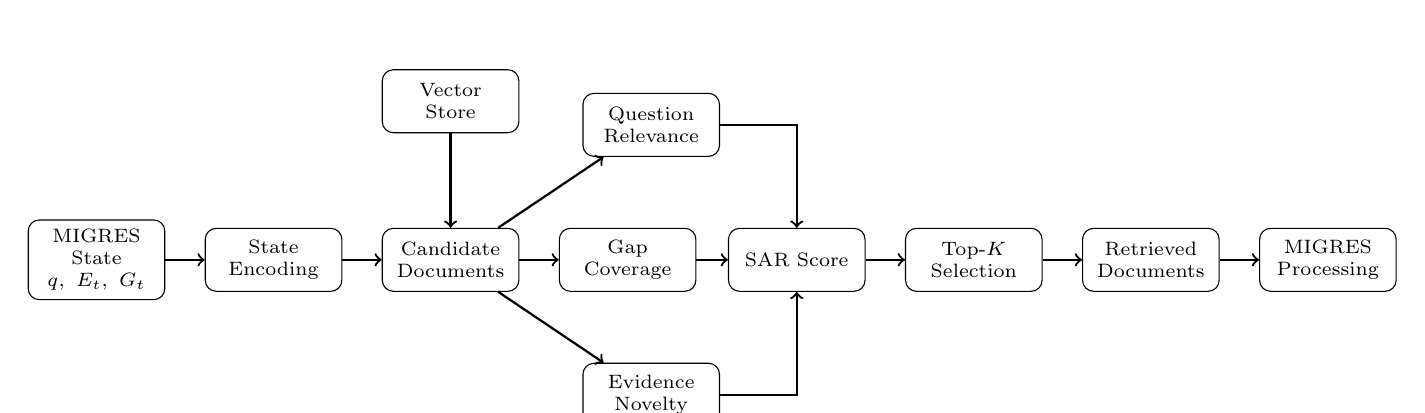
\begin{tikzpicture}[
    node distance=3mm and 5mm,
    box/.style={
        draw,
        rounded corners,
        align=center,
        minimum height=8mm,
        text width=15mm,
        font=\scriptsize
    },
    arrow/.style={
        ->,
        thick
    }
]

% Main flow
\node[box] (state) {MIGRES State\\$q,\ E_t,\ G_t$};

\node[box, right=of state] (encoding)
{State\\Encoding};

\node[box, right=of encoding] (candidates)
{Candidate\\Documents};

% SAR scoring components
\node[box, above right=9mm and 8mm of candidates] (relevance)
{Question\\Relevance};

\node[box, right=of candidates] (gap)
{Gap\\Coverage};

\node[box, below right=9mm and 8mm of candidates] (novelty)
{Evidence\\Novelty};

% Score and selection
\node[box, right=4mm of gap] (score)
{SAR Score};

\node[box, right=of score] (topk)
{Top-$K$\\Selection};

\node[box, right=of topk] (docs)
{Retrieved\\Documents};

\node[box, right=of docs] (processing)
{MIGRES\\Processing};

% Main flow
\draw[arrow] (state) -- (encoding);
\draw[arrow] (encoding) -- (candidates);

% Scoring branches
\draw[arrow] (candidates) -- (relevance);
\draw[arrow] (candidates) -- (gap);
\draw[arrow] (candidates) -- (novelty);

% Merge into SAR score
\draw[arrow] (relevance.east) -| (score.north);
\draw[arrow] (gap.east) -- (score.west);
\draw[arrow] (novelty.east) -| (score.south);

% Final flow
\draw[arrow] (score) -- (topk);
\draw[arrow] (topk) -- (docs);
\draw[arrow] (docs) -- (processing);

% Vector store input
\node[box, above=12mm of candidates]
(vector) {Vector Store};

\draw[arrow] (vector) -- (candidates);

\end{tikzpicture}

\caption{Architecture of the SAR Retrieval Module}
\label{fig:sar-module}
\end{figure}

\clearpage

\section{Experimental Setup and Execution Plan}

The experimental setup defines how the proposed system is configured, executed, and evaluated in practice. The experiments involve connecting the implemented modules into complete execution pipelines, preparing the required inputs and configurations, running the defined experimental conditions, and recording the outputs produced by each run. The setup is designed to ensure that the same procedures can be executed consistently across different experimental configurations, while preserving the results and intermediate information required for subsequent analysis and comparison.

\begin{figure}[H]
\centering
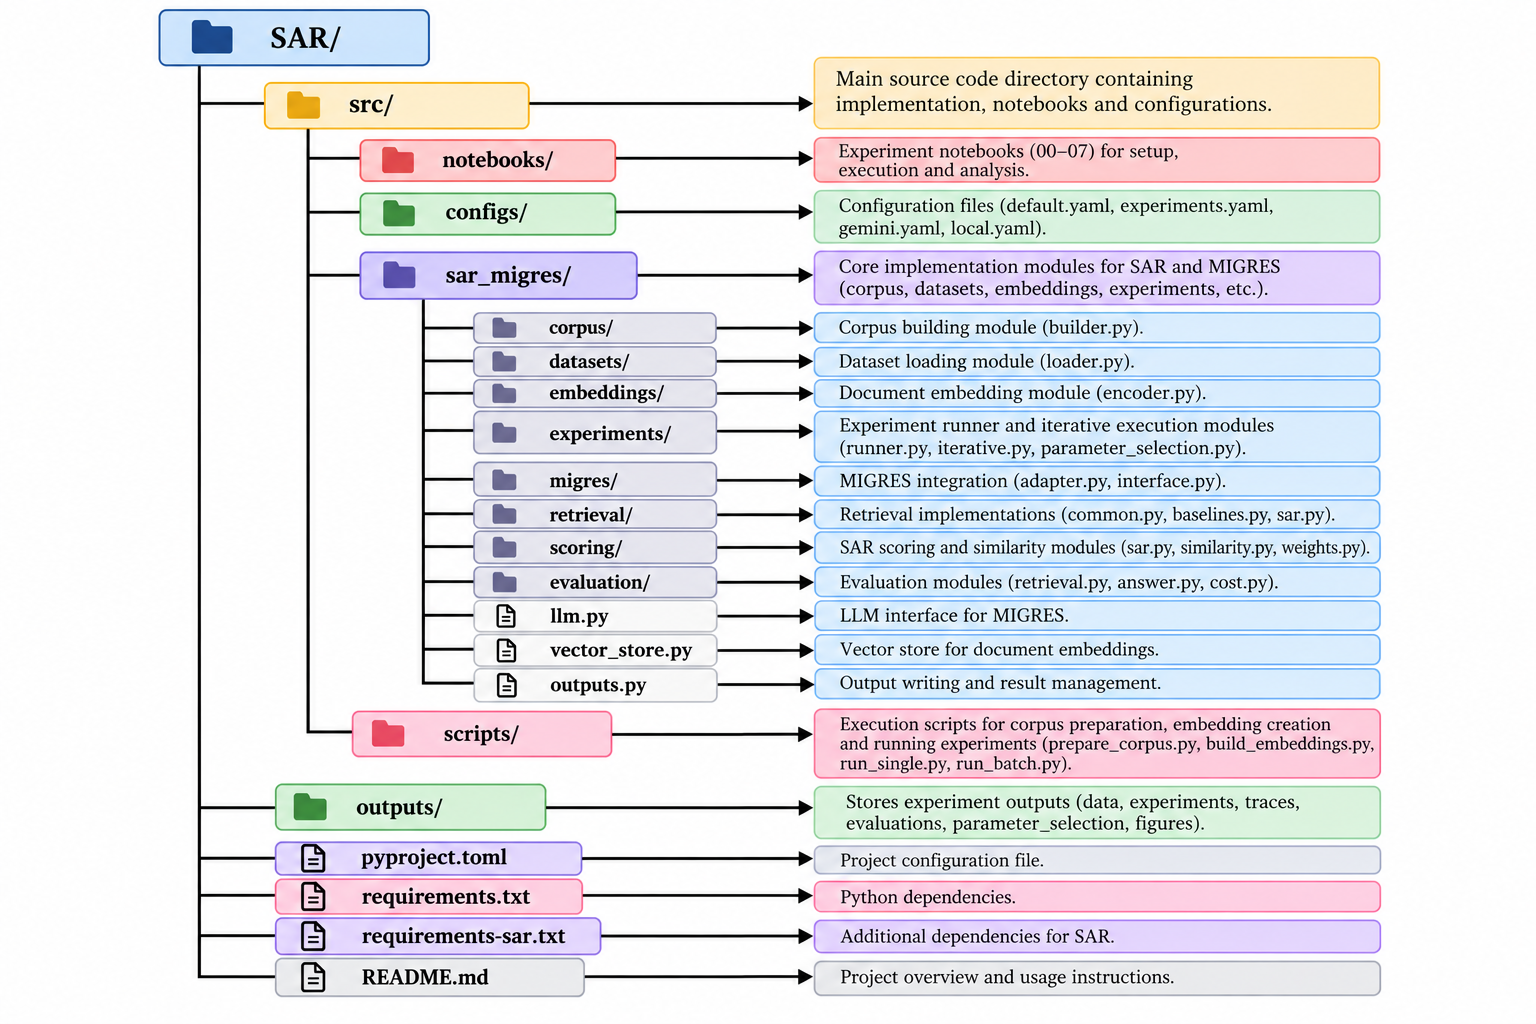
\includegraphics[width=0.95\textwidth]{ps.png}
\caption{Project Structure of the SAR--MIGRES Implementation}
\label{fig:project-structure}
\end{figure}

\subsection{Integration of MIGRES with State-Aware Retrieval}

The official MIGRES code is used as it is, without any change to its
files. The connection between MIGRES and SAR is made in one file,
\texttt{adapter.py}. This file does the following:

\begin{itemize}[leftmargin=1.8em,itemsep=3pt]
    \item \textbf{Loads MIGRES.} MIGRES has a class called
    \texttt{RetGBatched} in its file \texttt{pipeline.py}, which
    controls the retrieval steps. \texttt{adapter.py} reads this class
    so that it can be used in our project.

    \item \textbf{Creates a new class.} \texttt{adapter.py} creates a
    new class based on \texttt{RetGBatched}. The new class works
    exactly like the original one, except for two functions that are
    replaced.

    \item \textbf{Replaces \texttt{search()}.} MIGRES calls this
    function whenever it needs documents. In the new class, it sends
    the current question, the evidence collected so far, and the
    missing information to the SAR retriever instead of the MIGRES
    searcher.

    \item \textbf{Replaces \texttt{askGPT()}.} MIGRES calls this
    function to get a response from the language model. In the new
    class, it sends the prompt to \texttt{llm.py}, which calls the
    model and returns the response.
\end{itemize}

The retrieval is done in two files. In \texttt{sar.py} (retrieval), the
function \texttt{retrieve()} of \textbf{StateAwareRetriever} receives
the question, evidence, and missing information from \texttt{search()}.
It scores the documents using \texttt{score\_components()} and
\texttt{sar\_score()} from \texttt{sar.py} (scoring) and selects the
Top-$K$ documents. These are returned to MIGRES through
\texttt{adapter.py}, and MIGRES continues its iterative process as
usual. Therefore, SAR replaces only the document retrieval step of MIGRES,
and the rest of the iterative process is unchanged.

\subsection{Code-Level Architecture}

\begin{figure}[H]
\centering
\resizebox{\textwidth}{!}{%
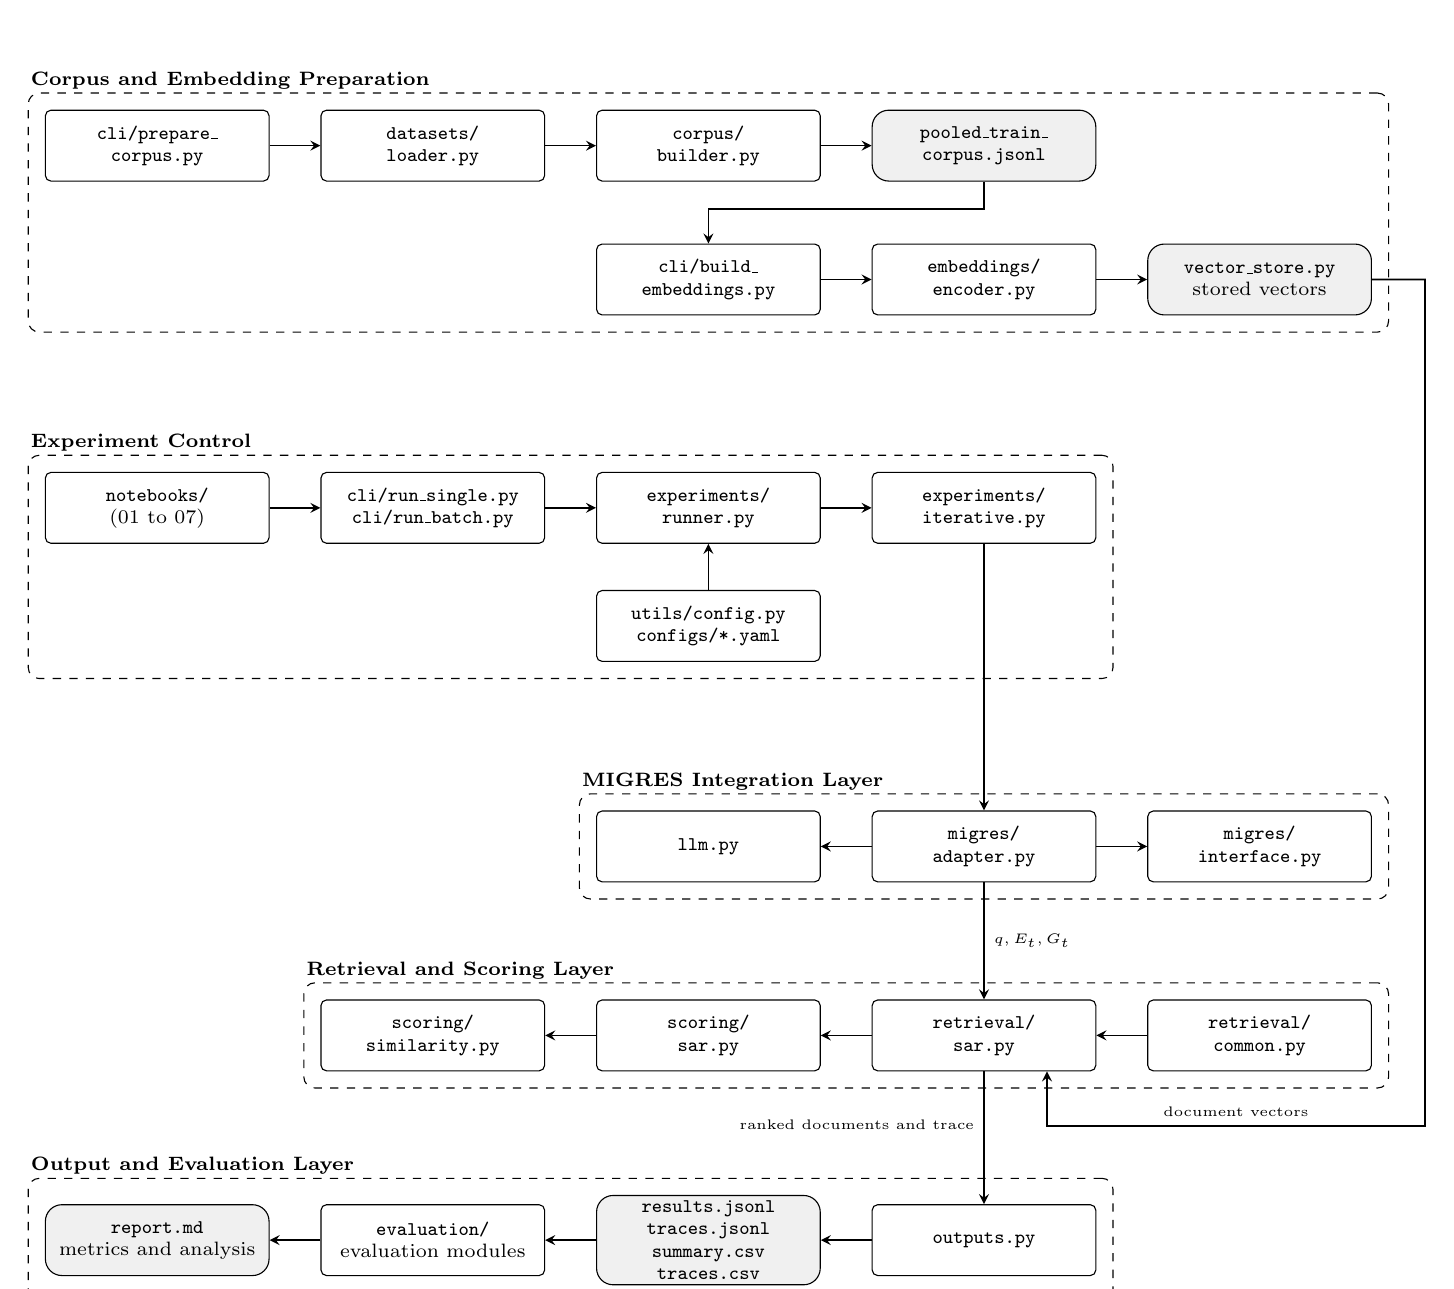
\begin{tikzpicture}[
    py/.style={
        draw,
        rounded corners=2pt,
        align=center,
        minimum height=9mm,
        text width=27mm,
        inner sep=2pt,
        font=\scriptsize
    },
    dt/.style={
        py,
        rounded corners=6pt,
        fill=black!6
    },
    ar/.style={
        ->,
        >=stealth,
        line width=0.6pt
    },
    grp/.style={
        draw,
        dashed,
        rounded corners=4pt,
        inner sep=6pt
    }
]

% ================= Corpus and Embedding Preparation =================
\node[py] (prep)       at (0,0)     {\texttt{cli/prepare\_}\\\texttt{corpus.py}};
\node[py] (loader)     at (3.5,0)   {\texttt{datasets/}\\\texttt{loader.py}};
\node[py] (builder)    at (7,0)     {\texttt{corpus/}\\\texttt{builder.py}};
\node[dt] (corpus)     at (10.5,0)  {\texttt{pooled\_train\_}\\\texttt{corpus.jsonl}};

\node[py] (embedbuild) at (7,-1.7)  {\texttt{cli/build\_}\\\texttt{embeddings.py}};
\node[py] (encoder)    at (10.5,-1.7){\texttt{embeddings/}\\\texttt{encoder.py}};
\node[dt] (store)      at (14,-1.7) {\texttt{vector\_store.py}\\stored vectors};

\draw[ar] (prep)--(loader);
\draw[ar] (loader)--(builder);
\draw[ar] (builder)--(corpus);
\draw[ar] (corpus.south) -- ++(0,-0.35) -| (embedbuild.north);
\draw[ar] (embedbuild)--(encoder);
\draw[ar] (encoder)--(store);

\node[grp,
    fit=(prep)(loader)(builder)(corpus)(embedbuild)(encoder)(store),
    label={[font=\scriptsize\bfseries,anchor=south west,inner sep=1pt]
    north west:Corpus and Embedding Preparation}] (gA) {};

% ================= Experiment Control =================
\node[py] (notebooks) at (0,-4.6)
{\texttt{notebooks/}\\(01 to 07)};
\node[py] (cli)       at (3.5,-4.6)
{\texttt{cli/run\_single.py}\\\texttt{cli/run\_batch.py}};
\node[py] (runner)    at (7,-4.6)
{\texttt{experiments/}\\\texttt{runner.py}};
\node[py] (pipeline)  at (10.5,-4.6)
{\texttt{experiments/}\\\texttt{iterative.py}};
\node[py] (config)    at (7,-6.1)
{\texttt{utils/config.py}\\\texttt{configs/*.yaml}};

\draw[ar] (notebooks)--(cli);
\draw[ar] (cli)--(runner);
\draw[ar] (runner)--(pipeline);
\draw[ar] (config)--(runner);

\node[grp,
    fit=(notebooks)(cli)(runner)(pipeline)(config),
    label={[font=\scriptsize\bfseries,anchor=south west,inner sep=1pt]
    north west:Experiment Control}] (gB) {};

% ================= MIGRES Integration =================
\node[py] (llm)       at (7,-8.9)    {\texttt{llm.py}};
\node[py] (adapter)   at (10.5,-8.9) {\texttt{migres/}\\\texttt{adapter.py}};
\node[py] (interface) at (14,-8.9)   {\texttt{migres/}\\\texttt{interface.py}};

\draw[ar] (adapter)--(llm);
\draw[ar] (adapter)--(interface);

\node[grp,
    fit=(llm)(adapter)(interface),
    label={[font=\scriptsize\bfseries,anchor=south west,inner sep=1pt]
    north west:MIGRES Integration Layer}] (gC) {};

% ================= Retrieval and Scoring =================
\node[py] (sim)       at (3.5,-11.3)  {\texttt{scoring/}\\\texttt{similarity.py}};
\node[py] (score)     at (7,-11.3)    {\texttt{scoring/}\\\texttt{sar.py}};
\node[py] (retrieval) at (10.5,-11.3) {\texttt{retrieval/}\\\texttt{sar.py}};
\node[py] (common)    at (14,-11.3)   {\texttt{retrieval/}\\\texttt{common.py}};

\draw[ar] (common)--(retrieval);
\draw[ar] (retrieval)--(score);
\draw[ar] (score)--(sim);

\node[grp,
    fit=(sim)(score)(retrieval)(common),
    label={[font=\scriptsize\bfseries,anchor=south west,inner sep=1pt]
    north west:Retrieval and Scoring Layer}] (gD) {};

% ================= Output and Evaluation =================
\node[py] (outputs)   at (10.5,-13.9) {\texttt{outputs.py}};
\node[dt] (artifacts) at (7,-13.9)
{\texttt{results.jsonl}\\\texttt{traces.jsonl}\\\texttt{summary.csv}\\\texttt{traces.csv}};
\node[py] (eval)      at (3.5,-13.9)  {\texttt{evaluation/}\\evaluation modules};
\node[dt] (report)    at (0,-13.9)    {\texttt{report.md}\\metrics and analysis};

\draw[ar] (outputs)--(artifacts);
\draw[ar] (artifacts)--(eval);
\draw[ar] (eval)--(report);

\node[grp,
    fit=(outputs)(artifacts)(eval)(report),
    label={[font=\scriptsize\bfseries,anchor=south west,inner sep=1pt]
    north west:Output and Evaluation Layer}] (gE) {};

% ================= Cross-layer data flow =================
% control -> MIGRES adapter
\draw[ar] (pipeline.south) -- (adapter.north);

% state passed from the adapter to SAR retrieval
\draw[ar] (adapter.south) -- node[right,font=\tiny]{$q,E_t,G_t$} (retrieval.north);

% ranked documents and trace to the output layer
\draw[ar] (retrieval.south) -- node[pos=0.4,left,font=\tiny]{ranked documents and trace} (outputs.north);

% document vectors: routed along the right margin, so nothing is crossed
\draw[ar] (store.east) -- (16.1,-1.7) -- (16.1,-12.45)
    -- (11.3,-12.45) -- ([xshift=8mm]retrieval.south);
\node[font=\tiny,above] at (13.7,-12.45) {document vectors};

\end{tikzpicture}%
}
\caption{Code-Level Architecture of the SAR--MIGRES Implementation}
\label{fig:code-level-architecture}
\end{figure}

In summary, the code-level architecture maps the SAR--MIGRES design onto
the \texttt{sar\_migres} package, where each module has a single
responsibility. SAR is connected to MIGRES only through the adapter, so
the rest of the iterative pipeline remains unchanged.
%=================================================


\subsection{SAR Scoring and Retrieval Module}

The SAR scoring and retrieval module decides which documents are returned to MIGRES at each iteration. The scoring module (\texttt{scoring/sar.py}, \texttt{scoring/similarity.py}) evaluates each document against the current retrieval state, and the retrieval module (\texttt{retrieval/sar.py}) applies this scoring to the whole corpus and selects the Top-$K$ documents.

Given the question $q$, the information gaps $G_t$, the collected evidence $E_t$, and the stored document vectors, the scoring module computes three signals using the normalized cosine similarity $s(x,y)=\frac{1+\cos(x,y)}{2}$:
\[
R(d,q)=s(d,q), \qquad
C(d,G_t)=\frac{1}{|G_t|}\sum_{g_i\in G_t}s(d,g_i), \qquad
N(d,E_t)=1-\max_{e_j\in E_t}s(d,e_j),
\]
where $C=0$ if $G_t$ is empty and $N=1$ if $E_t$ is empty. The final score is
\[
S_t(d)=\alpha R(d,q)+\beta C(d,G_t)+\gamma N(d,E_t),
\]
with default weights $\alpha=0.4$, $\beta=0.3$, $\gamma=0.3$.

The retrieval module scores the document vectors in chunks and returns the $K=50$ highest-scoring documents, with ties broken by document id. The ranked documents and their scores are passed to MIGRES through \texttt{adapter.py} and saved in the retrieval trace.

\begin{figure}[H]
\centering
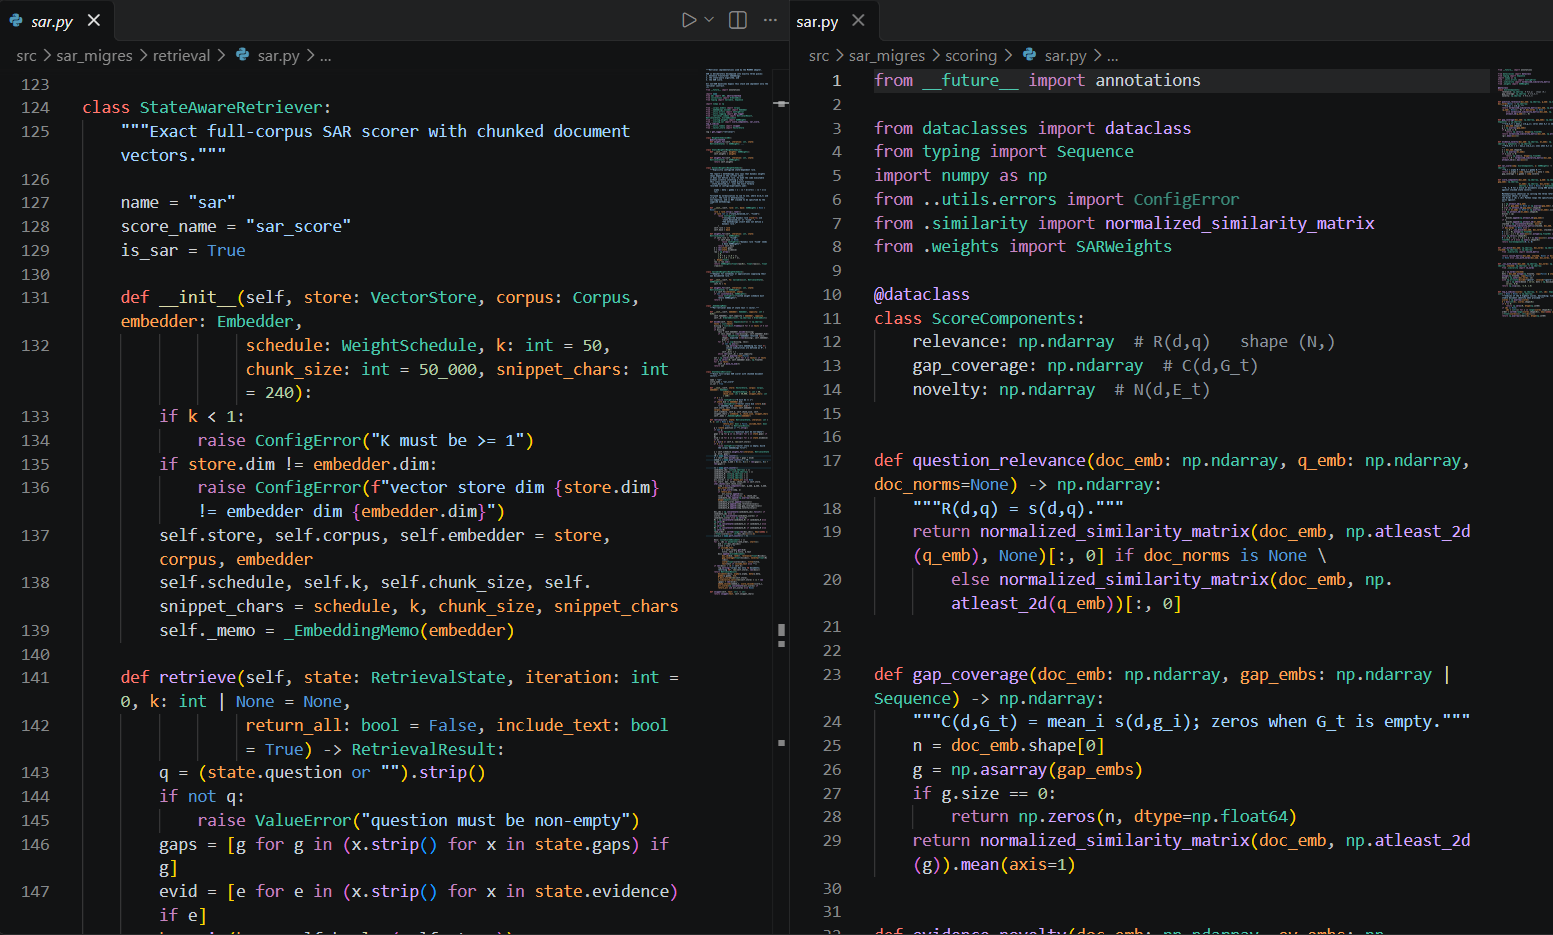
\includegraphics[width=0.95\textwidth]{sar.png}
\caption{Implementation of the SAR Scoring and Retrieval Module}
\label{fig:sar-scoring-retrieval-module}
\end{figure}
\clearpage
The following pseudocode shows how \textbf{score\_components()}, \textbf{sar\_score()}, and \textbf{StateAwareRetriever.retrieve()} work together.

\medskip
\noindent\begin{minipage}{\textwidth}
\noindent\rule{\textwidth}{0.8pt}\\[-2pt]
\noindent\textbf{Algorithm 7.1:} SAR Scoring and Retrieval\\[-6pt]
\noindent\rule{\textwidth}{0.4pt}

\noindent\textbf{Input:} question $q$, gaps $G_t$, evidence $E_t$,
document vector store $\mathcal{V}$, weights $(\alpha,\beta,\gamma)$, depth $K$\\
\noindent\textbf{Output:} ranked Top-$K$ documents $T_t$ with $R$, $C$, $N$, $S_t$

\medskip
\noindent\textbf{Procedure} \textsc{ScoreChunk}$(B,q,G_t,E_t)$

\noindent\begin{tabular}{@{}r@{\hspace{0.9em}}l@{}}
1: & $S \leftarrow s(B,[q;G_t;E_t])$ using one matrix product \\
2: & $R \leftarrow$ column of $S$ for $q$ \\
3: & \textbf{if} $G_t=\emptyset$ \textbf{then} $C\leftarrow0$
\textbf{else} $C\leftarrow$ mean of the gap columns of $S$ \\
4: & \textbf{if} $E_t=\emptyset$ \textbf{then} $N\leftarrow1$
\textbf{else} $N\leftarrow1-$ max of the evidence columns of $S$ \\
5: & $S_t\leftarrow\alpha R+\beta C+\gamma N$ \\
6: & \textbf{return} $(R,C,N,S_t)$
\end{tabular}

\medskip
\noindent\textbf{Procedure} \textsc{Retrieve}$(q,G_t,E_t,\mathcal{V},K)$

\noindent\begin{tabular}{@{}r@{\hspace{0.9em}}l@{}}
1: & Remove empty strings from $G_t$ and $E_t$ \\
2: & $K\leftarrow\min(K,|\mathcal{V}|)$ \\
3: & Encode $q$, $G_t$, and $E_t$ \\
4: & $L \leftarrow \emptyset$ \\
5: & \textbf{for each} chunk $B$ of document vectors in $\mathcal{V}$ \textbf{do} \\
6: & \hspace{1.5em}$(R,C,N,S_t)\leftarrow$ \textsc{ScoreChunk}$(B,q,G_t,E_t)$ \\
7: & \hspace{1.5em}Add the $K$ highest-scoring documents of $B$ to $L$
(ties broken by document id) \\
8: & \textbf{end for} \\
9: & Sort $L$ by $S_t$ (descending), then by document id \\
10: & $T_t\leftarrow$ first $K$ documents of $L$ \\
11: & \textbf{return} $T_t$
\end{tabular}

\noindent\rule{\textwidth}{0.8pt}
\end{minipage}

\medskip
In summary, the scoring module turns the retrieval state into a score for each document, and the retrieval module uses these scores to select the documents that MIGRES receives at the next iteration.
\subsection{Notebooks Used for Experimentation}

The experiments are executed in Google Colab through notebooks that serve as thin interfaces to the shared implementation in \texttt{src/sar\_migres}. The notebooks do not contain the retrieval algorithm. They call the same modules for SAR and for the baseline methods, which ensures that all methods are run and recorded under identical conditions. Notebook~00 prepares the Colab environment, and notebooks 01 to 07 correspond to the experiments described in Section~5.6. The experimental settings, including the SAR weights, datasets, MIGRES parameters, and LLM configuration, are specified in the YAML files under \texttt{src/configs/}.

\begin{table}[H]
\centering
\caption{Experiment Notebooks and Their Mapping to the Experimental Design}
\label{tab:impl-notebooks}
\renewcommand{\arraystretch}{1.15}
\begin{tabular}{|p{0.35in}|p{2.2in}|p{1.45in}|p{2.0in}|}
\hline
\textbf{No.} & \textbf{Notebook} & \textbf{Experiment (Section 5.6)} & \textbf{Purpose} \\
\hline
00 & \texttt{00\_colab\_setup.ipynb} & Not an experiment & Sets up the environment for Google Colab execution. \\
\hline
01 & \texttt{01\_parameter\_\allowbreak hyperparameter\_\allowbreak selection.ipynb} & 5.6.1 Hyperparameter Selection & Selects the SAR weighting parameters. \\
\hline
02 & \texttt{02\_baseline\_\allowbreak comparison.ipynb} & 5.6.2 Baseline Comparison & Compares SAR with the baseline retrievers. \\
\hline
03 & \texttt{03\_ablation\_\allowbreak study.ipynb} & 5.6.3 Ablation Study & Evaluates the contribution of each SAR component. \\
\hline
04 & \texttt{04\_retrieval\_\allowbreak performance.ipynb} & 5.6.4 Retrieval Performance Evaluation & Calculates retrieval metrics from completed runs. \\
\hline
05 & \texttt{05\_iterative\_\allowbreak state\_\allowbreak analysis.ipynb} & 5.6.5 Iterative State Analysis & Analyzes retrieval behavior across iterations using the stored traces. \\
\hline
06 & \texttt{06\_downstream\_\allowbreak rag\_\allowbreak robustness.ipynb} & 5.6.6 Downstream RAG and Robustness Evaluation & Evaluates downstream answer performance and robustness. \\
\hline
07 & \texttt{07\_computational\_\allowbreak cost.ipynb} & 5.6.7 Computational Cost Analysis & Measures retrieval and execution cost. \\
\hline
\end{tabular}
\end{table}

\subsection{Execution Output and Result Format}

Every experimental run saves its outputs to a separate run folder inside the output directory of its experiment, for example \texttt{outputs/experiments/02\_baseline\_comparison/runs/<run\_id>/}. The files are written during execution and are stored as JSON, JSONL, and CSV files for further processing, as a Markdown report for reading, and as a log file for the run. Question-level results and iteration-level retrieval traces are stored separately, so answer analysis and retrieval analysis can be performed independently.

Parameter selection saves two additional files in \texttt{outputs/experiments/01\_parameter\_selection/}. The first is the selected SAR weights, which are frozen and read by the later experiments. The second is the log of all tuning trials.

The evaluation metrics are not saved as separate files. They are calculated by the evaluation modules from the saved run files and shown in the notebook output. These include the retrieval metrics, iterative analysis, answer metrics, and computational cost.

\begin{table}[H]
\centering
\caption{Outputs Saved for Each Experimental Run}
\label{tab:impl-output-files}
\renewcommand{\arraystretch}{1.15}
\begin{tabular}{|p{1.45in}|p{0.95in}|p{3.7in}|}
\hline
\textbf{Output} & \textbf{Format} & \textbf{Data stored} \\
\hline
Question results & JSONL & Final answer, gold answer, run status, execution time, and LLM usage for each question. \\
\hline
Retrieval traces & JSONL & For each iteration: information gaps, collected evidence, ranked documents with their $R$, $C$, $N$ and final scores, SAR weights, and retrieval timing. \\
\hline
Trace table & CSV & Flattened version of the traces with one row per retrieved document, used for tabular analysis. \\
\hline
Summary table & CSV & One row per question with status, number of retrieval iterations, final answer, execution time, and LLM usage. \\
\hline
Configuration and metadata & JSON & Configuration used for the run, together with run information such as the retriever, dataset, corpus, models, and warnings. \\
\hline
Run report & Markdown & Readable summary of the run, with the retrieved documents and scores for each iteration. \\
\hline
Execution log & LOG & Messages written during the run, such as progress, warnings, and errors. \\
\hline
\end{tabular}
\end{table}


\section{Conclusion}
% ============================================================

This chapter described the implementation of the proposed SAR-MIGRES
system and its supporting experimental infrastructure. The SAR retrieval
procedure, document embedding and vector-store preparation, MIGRES
integration, baseline retrieval methods, and evaluation components have
been implemented in the shared Python source and experiment notebooks.

The system is now prepared for the final experimental runs. The
implementation and evaluation pipeline are in place, while the final
execution and generation of experimental results remain pending.

\label{ch:7:end}

\clearpage

% ============================================================
% CHAPTER 7 -- APPLICATIONS
% ============================================================

\addcontentsline{toc}{chapter}{8. APPLICATIONS}
\chaptertitle{8}{APPLICATIONS}
\label{ch:8}
\justifying

\begin{enumerate}[leftmargin=0.30in,itemsep=0.12in]

\item
\textbf{Complex Question Answering:} SAR can support AI systems in answering complex questions where the required information is spread across multiple documents and cannot be obtained in a single retrieval step.

\item
\textbf{Multi-Step Information Retrieval:} SAR can be applied to systems that search for information repeatedly, helping each retrieval step focus on the information that has not yet been obtained.

\item
\textbf{Research and Knowledge Discovery:} SAR can help collect information from large document collections by prioritizing useful and complementary evidence instead of repeatedly retrieving similar content.

\item
\textbf{Evidence-Based RAG Applications:} SAR can be integrated into RAG-based applications that need to build a complete set of evidence before generating an answer, such as question answering, document analysis, and knowledge-based assistants.

\end{enumerate}
\clearpage


% ============================================================
% CHAPTER 8
% GANTT CHART
% ============================================================

\setcounter{table}{0}
\renewcommand{\thetable}{9.\arabic{table}}
\renewcommand{\theHtable}{chapter9.\arabic{table}}
\setcounter{figure}{0}
\renewcommand{\thefigure}{9.\arabic{figure}}
\renewcommand{\theHfigure}{chapter9.\arabic{figure}}

\addcontentsline{toc}{chapter}{9. GANTT CHART}

\chaptertitle{9}{GANTT CHART}
\label{ch:9}

\begin{figure}[H]
\centering
\vspace{0.15in}
\IfFileExists{gantt_chart.png}{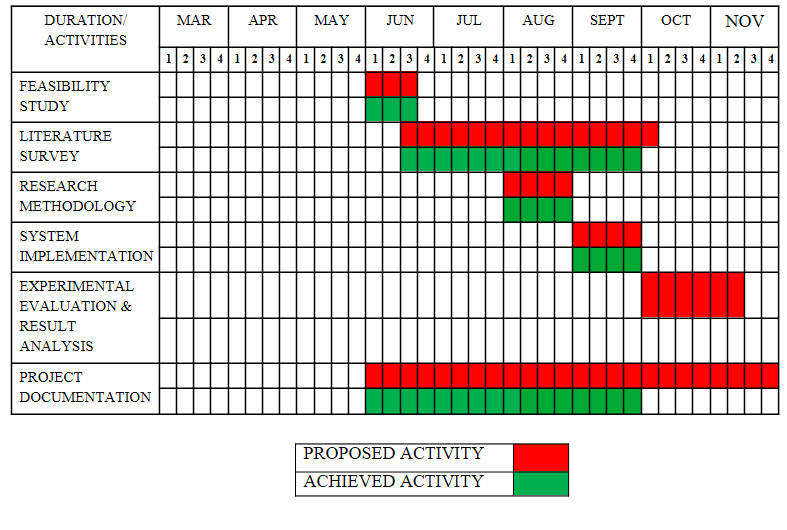
\includegraphics[width=0.95\textwidth]{gantt_chart.png}}{\fbox{\rule{0pt}{2.5in}\rule{5.5in}{0pt}}}
\caption{Gantt Chart}
\label{fig:gantt}
\end{figure}

\clearpage

% ============================================================
% CHAPTER 9
% CONCLUSION
% ============================================================

\addcontentsline{toc}{chapter}{10. CONCLUSION}

\chaptertitle{10}{CONCLUSION}
\label{ch:10}

\justifying

This project presents \textbf{State Aware Retrieval (SAR)} as a
direct retrieval method within the MIGRES framework. SAR uses the
current question, the information gaps, and the previously collected
evidence to guide document selection from the complete document corpus.
The selected documents are then passed to MIGRES for filtering, evidence
extraction, and further state updates.

The study will examine whether making retrieval aware of the current
information state can improve the quality and usefulness of the retrieved
evidence during iterative retrieval. The contribution of each state
signal will be studied through ablation experiments, while comparisons
with established retrieval methods will measure the overall retrieval
performance of SAR. The effect on final RAG performance, behavior across
iterations, robustness, and computational cost will also be evaluated.

Overall, this work provides a clear framework for testing whether
State Aware Retrieval can make iterative retrieval more focused on the
information that is relevant, still missing, and not already covered by
previous evidence. The main MIGRES framework remains unchanged, so the
study can directly examine the effect of the proposed retrieval
method. The final experimental results will determine the effectiveness
and practical value of SAR for iterative retrieval-augmented generation.

\clearpage

% ============================================================
% REFERENCES
% ============================================================

\addcontentsline{toc}{chapter}{REFERENCES}

\righttitle{REFERENCES}
\label{ch:refs}

\renewcommand{\bibname}{}

\bibliographystyle{IEEEtran}
\bibliography{citation}

\end{document}